\documentclass[french, 12pt]{article}

%-------------------------------------------------------------------------------
\usepackage[a4paper,top=2cm,bottom=2cm,left=2cm,right=2cm,marginparwidth=1.75cm]{geometry}
\usepackage{amsmath,amsfonts,amssymb,amsthm}
\usepackage[french]{babel}
\usepackage[utf8]{inputenc}
\usepackage[T1]{fontenc}
\usepackage{enumerate}
\usepackage{natbib}
\usepackage{graphicx}
\usepackage{xspace}
\usepackage{color,xcolor}
\usepackage{tikz}
\usepackage{remreset}
\usepackage{url}
\usepackage{boites}
% \usepackage{extsizes} % Permet \documentclass[french, 14pt]{extreport}
% \usepackage[a4paper,top=1cm,bottom=2cm,left=1cm,right=1cm,marginparwidth=.75cm]{geometry}
% \usepackage{minitoc}

\graphicspath{{../Figures/}}
% Environnement
\newtheorem{theorem}{Théorème}
\newtheorem{definition}{Définition}
\newtheorem{lemma}{Lemme}
\newtheorem{proposition}{Proposition}
\newtheorem*{theorem*}{Théorème}
\newtheorem*{definition*}{Définition}
\newtheorem*{proposition*}{Proposition}
\newtheorem*{corollary*}{Corollaire}
\newtheorem*{assumption*}{Hypothèse}
\newtheorem*{algorithm*}{Algorithme}
\newtheorem*{lemma*}{Lemme}
\newtheorem*{remark*}{Remarque}
\newtheorem*{exercise*}{Exercice}
\newtheorem{exercise}{Exercice}
\newcommand{\remark}{\bigskip\noindent\textbf{\textsl{Remarque.}}\xspace}
\newcommand{\remarks}{\bigskip\noindent\textbf{\textsl{Remarques.}}\xspace}
\newcommand{\parSR}[1]{\paragraph*{\textsl{#1}}\xspace}
\renewcommand{\proof}{\bigskip\noindent\underline{\textsl{Démonstration}.}\xspace}
\newcommand{\eproof}{$\blacksquare$}

% Effets, couleurs
\newcommand{\emphase}[1]{\textcolor{red}{#1}}
\newcommand{\demoProp}[1]{\noindent{\textbf{\textsl{Démonstration de la proposition \ref{#1} :}}}}
\newcommand{\itemdot}{\textbullet}

% Moments
\DeclareMathOperator{\Esp}{\mathbb{E}}
\DeclareMathOperator{\diag}{diag}
\DeclareMathOperator{\Cov}{\mathbb{C}ov}
\DeclareMathOperator{\tr}{tr}
\DeclareMathOperator{\Var}{\mathbb{V}}
\let\Pr\relax\DeclareMathOperator{\Pr}{\mathbb{P}}
\renewcommand{\d}{\text{d}}

% R, N, ...
\newcommand{\cst}{\text{cst}}
\newcommand{\Cbb}{\mathbb{C}}
\newcommand{\Ibb}{\mathbb{I}}
\newcommand{\Nbb}{\mathbb{N}}
\newcommand{\Rbb}{\mathbb{R}}
\newcommand{\Zbb}{\mathbb{Z}}

% Indicateurs

% Lois et ensembles
\newcommand{\Acal}{\mathcal{A}}
\newcommand{\Bcal}{\mathcal{B}}
\newcommand{\Ccal}{\mathcal{C}}
\newcommand{\Ecal}{\mathcal{E}}
\newcommand{\Gcal}{\mathcal{G}}
\newcommand{\Ical}{\mathcal{I}}
\newcommand{\Lcal}{\mathcal{L}}
\newcommand{\Mcal}{\mathcal{M}}
\newcommand{\Ncal}{\mathcal{N}}
\newcommand{\Pcal}{\mathcal{P}}
\newcommand{\Rcal}{\mathcal{R}}
\newcommand{\Scal}{\mathcal{S}}
\newcommand{\Ucal}{\mathcal{U}}
\newcommand{\Xcal}{\mathcal{X}}
\newcommand{\Ycal}{\mathcal{Y}}

% Comments
\newcommand{\SR}[2]{\textcolor{gray}{#1}\textcolor{red}{#2}}
\newcommand{\todo}[1]{\textcolor{red}{\`A faire~: {\sl #1}}}
\newcommand{\dessin}[1]{
\begin{center}\framebox{\begin{minipage}{\textwidth}
  \textcolor{purple}{#1}
\end{minipage}}\end{center}
\bigskip
}
\newcommand{\progres}[1]{
\begin{center}\framebox{\begin{minipage}{\textwidth}
  \textcolor{blue}{{\sl #1}}
\end{minipage}}\end{center}
\bigskip
}
\newcommand{\solution}[1]{
\begin{center}\framebox{\begin{minipage}{\textwidth}
  \noindent{\sl Solution :}
  #1
\end{minipage}}\end{center}
\bigskip
}
% \newcommand{\exemple}[1]{
% \begin{center}\framebox{\begin{minipage}{\textwidth}
%   \parSR{Exemple.}
%   #1
% \end{minipage}}\end{center}
% \bigskip
% }
\newcommand{\exemple}[1]{
\begin{breakbox}
  \parSR{Exemple.}
  #1
\end{breakbox}
\bigskip
}

\newcommand{\SRcorrect}[2]{\textcolor{gray}{#1}\textcolor{blue}{#2}}
\newcommand{\SRcomment}[1]{\textcolor{blue}{[{\sl SR: #1}]}}



% Proposition numbering
% \numberwithin{proposition}{section}
\numberwithin{exercise}{subsection}
\numberwithin{equation}{subsection}

\pagestyle{myheadings}
\markright{ENS Paris, L3 Biologie \hfill Année 2022–23 \hfill Mathématiques I \hfill }

% Suppression des solutions
% \renewcommand{\solution}[1]{}

%-------------------------------------------------------------------------------
%-------------------------------------------------------------------------------
\title{{Ce qu'un biologiste doit savoir en mathématiques : \\ Exercices}}
\author{SR (inspiré d'AL)}
\date{\today}

%-------------------------------------------------------------------------------
%-------------------------------------------------------------------------------
\begin{document}
%-------------------------------------------------------------------------------
%-------------------------------------------------------------------------------

\maketitle
\tableofcontents

\newpage \section{Algèbre linéaire} %-------------------------------------------------------------------------------
\subsection{Exemples de matrices et déterminants}%-------------------------------------------------------------------------------

%-------------------------------------------------------------------------------
\subsubsection{Calculs de déterminants}
Calculer les déterminants des matrices suivantes 
\begin{align*}
%     A_1 & = \left[\begin{array}{rrr}
%       2 & -1 & 3 \\ 2 & -1 & 6 \\ -2 & 1 & 0
%       \end{array}\right], &
%     %
%     A_2 & = \left[\begin{array}{rrr}
%       2 & -1 & 3 \\ 2 & -1 & 6 \\ 1 & 0  & 2
%       \end{array}\right], \\
%     %
  A & = \left[\begin{array}{rrr}
    1 & 1 & 0 \\ -5 & -2 & 5 \\ -1 & 0 & 2
    \end{array}\right], &
  B & = \left[\begin{array}{rrr}
    -1 & 3 & 1 \\ 0 & 2 & 1 \\ 2 & 1 & 2
    \end{array}\right].  
\end{align*}

\solution{
  \begin{align*}
%     |A_1| & = 0 & & \text{colonne } 1 = -2 \text{ colonne } 2 \\
%     %
%     |A_2| & = 1 \times (-3) + 2 \times 0 = -3 & & \text{développement / dernière ligne} \\
    %
    |A| & = 1 \times (-4) - 1 \times (-5) = 1 & & \text{développement / première ligne} \\
    %
    |B| & = -1 \times 3 + 2 \times 1 = -1 & &  \text{développement / première colonne}
  \end{align*}
}

%-------------------------------------------------------------------------------
\subsubsection{Matrices diagonalisables ?}
Déterminer le polynôme caratéristique des matrices suivantes et en déduire si elles sont diagonalisables
\begin{align*}
  A & = \left[\begin{array}{rrr}
    2 & -1 & 3 \\ 2 & -1 & 6 \\ 1 & 0  & 2
    \end{array}\right], &
  B & = \left[\begin{array}{rrr}
    1 & 1 & 0 \\ -5 & -2 & 5 \\ -1 & 0 & 2
    \end{array}\right].
\end{align*}
  
\solution{
  \begin{description}
    \item[$A$ :] on a
    \begin{align*}
        P_A(\lambda) 
        = \left| \begin{array}{rrr}
          2 - \lambda & -1 & 3 \\ 2 & -1 - \lambda & 6 \\ 1 & 0  & 2 - \lambda 
          \end{array}\right|
        = -\lambda^3 + 3 \lambda^2 + \lambda - 3
        = -(\lambda - 3) (\lambda - 1) (\lambda + 1).
    \end{align*}
    Les valeurs propres sont donc $3$, $1$ et $-1$ qui sont toutes réelles et distinctes, donc $A$ est diagonalisable.
    \item[$B$ :] on a
    \begin{align*}
        P_B(\lambda) 
        = \left| \begin{array}{rrr}
            1 - \lambda & 1 & 0 \\ -5 & -2 - \lambda & 5 \\ -1 & 0 & 2 - \lambda
          \end{array}\right|
        = - \lambda^3 + \lambda^2 - \lambda + 1
        = - (\lambda-1) (\lambda^2 + 1).
    \end{align*}
    Les valeurs propres sont donc $1$, $i$ et $-i$ qui ne sont pas toutes réelles, donc $B$ n'est pas diagonalisable.
  \end{description}
}

%-------------------------------------------------------------------------------
\subsubsection{Matrice paramétrée}
Soit la matrice
\begin{align*}
  A & = \left[\begin{array}{rrr}
    1 & 4 & 2 \\ 0 & \alpha & 0 \\ 1 & 1 & 0
    \end{array}\right]
\end{align*}
\begin{enumerate}
  \item Déterminer son polynôme caractéristique.
  \solution{En développant par rapport à la 2ème ligne, on obtient
    $$
    P_A(\lambda) 
    = (\alpha - \lambda) 
      \left| \begin{array}{cc} 1 - \lambda & 2 \\1 & - \lambda \end{array} \right|
    = (\alpha - \lambda) (\lambda^2 - \lambda - 2)
    = (\alpha - \lambda) (\lambda - 2 ) ( \lambda + 1).
    $$
  }
  \item En déduire ses valeurs propres et sa valeur propre dominante en fonction de $\alpha$.
  \solution{Les valeurs propres de $A$ sont donc $\{\alpha, 2, -1\}$. La valeur propre dominante    est donc $\max(\alpha, 2)$.}
  \item A quelle condition sur $\alpha$ $A$ est-elle diagonalisable ?
  \solution{
    \begin{description}
    \item[$\alpha \notin \{-1, 2\}$:] les 3 valeurs propres sont réelles et distinctes donc $A$ est diagonalisable.
    \item[$\alpha = 2$:] $2$ est alors raçine double de $P_A(\lambda)$ et ses vecteurs propres associés sont solutions de 
    $$
    \left\{ \begin{array}{rcl}  
            u_1 + 4 u_2 + 2 u_3 & = & 2 u_1 \\
            2 u_2 & = & 2 u_2 \\
            u_1 + u_2 & = & 2 u_3 
            \end{array} \right.
    \quad \Leftrightarrow \quad
    \left\{ \begin{array}{rcl}  
            2 u_1 + 5 u_2 & = & 2 u_1 \\
            u_1 + u_2 & = & 2 u_3 
            \end{array} \right.         
    \quad \Leftrightarrow \quad
    \left\{ \begin{array}{rcl}  
            u_2 & = & 0 \\
            u_1 & = & 2 u_3 
            \end{array} \right.         
    $$
    qui définit un sous-espace propre de dimension 1 : $A$ n'est donc pas diagonalisable.
    \item[$\alpha = -1$:] $-1$ est alors raçine double de $P_A(\lambda)$ et ses vecteurs propres associés sont solutions de 
    $$
    \left\{ \begin{array}{rcl}  
            u_1 + 4 u_2 + 2 u_3 & = & - u_1 \\
            2 u_2 & = & - u_2 \\
            u_1 + u_2 & = & - u_3 
            \end{array} \right.
    \quad \Leftrightarrow \quad
    \left\{ \begin{array}{rcl}  
            u_1 + 2 u_3 & = & - u_1 \\
            u_2 & = & 0 \\
            u_1& = & - u_3 
            \end{array} \right.
    \quad \Leftrightarrow \quad
    \left\{ \begin{array}{rcl}  

    u_2 & = & 0 \\
            u_1 & = & - u_3 
            \end{array} \right.
    $$
    qui définit un sous-espace propre de dimension 1 : $A$ n'est donc pas diagonalisable.
  \end{description}
  }
\end{enumerate}


%-------------------------------------------------------------------------------
\subsection{Propriétés générales du déterminant}%-------------------------------------------------------------------------------

%-------------------------------------------------------------------------------
\subsubsection{Polynôme caractéristique et trace}
On rappelle que la trace $\tr(A)$ d'une matrice carrée $A \in \Mcal_n$ est la somme de ses termes diagonaux : $\tr(A) = \sum_{i=1}^n a_{ii}$.
\begin{enumerate}
  \item Montrer que le coefficient d'ordre $n-1$ du polynôme caratéristique de $A$ (noté $P_A$) vaut
  $$
  [\lambda^{n-1}] P_A(\lambda) = (-1)^{n-1} \tr(A).
  $$
  On pourra procéder par récurrence.
  \solution{
    On vérifie facilement que la propriété est vraie pour $n=2$. En la supposant vraie au rang $n-1$, on peut calculer le polynôme caractéristique de $A \in \Mcal_n$ en développant par la dernière ligne : 
    $$
    P_A(\lambda) = 
    \left| A - \lambda I\right|
    = \sum_{j=1}^{n-1} (-1)^{n+j} a_{nj} \left| (A - \lambda I)^{(n, j)} \right|
    + (a_{nn} -\lambda) \left| (A - \lambda I)^{(n, n)} \right|
    $$
    en notant $B^{(i,j)}$ la matrice $B$ privée de sa $i$ème ligne et $j$ème colonne. On peut alors remarquer que les termes de la première somme sont tous de degré au plus $n-2$ et que $\left|(A - \lambda I)^{(n, n)} \right| = P_{A^{(n, n)}}(\lambda)$. On a donc, en notant $Q_m$ un polynôme quelconque de degré inférieur ou égal à $m$,
    \begin{align*}
      P_A(\lambda) 
      & = (a_{nn} -\lambda) P_{A^{(n, n)}}(\lambda) + Q_{n-2}(\lambda) \\
      & = (a_{nn} -\lambda) \left( (-1)^{n-1} \lambda^{n-1} + (-1)^{n-2} \tr(A^{(n, n)}) \lambda^{n-2} + Q_{n-3}(\lambda) \right) + Q_{n-2}(\lambda)
      & & (\text{par hypothèse}) \\
      & = - \lambda (-1)^{n-1} \lambda^{n-1} 
      + a_{nn} (-1)^{n-1} \lambda^{n-1} 
      - \lambda (-1)^{n-2} \tr(A^{(n, n)}) \lambda^{n-2}
      + Q'_{n-2}(\lambda) \\
      & = (-1)^n \lambda^n + (-1)^{n-1} \underset{\tr(A)}{\underbrace{(a_{nn} + \tr(A^{(n, n)})}} \lambda^{n-1} + Q'_{n-2}(\lambda)
    \end{align*}
    donc
    $$
    [\lambda^{n-1}] P_A(\lambda) = (-1)^{n-1} \tr(A).
    $$
  }
  \item En déduire que la trace est égale à la somme des raçines $\{\lambda_1, \dots \lambda_n\}$ de $P_A(\lambda)$ :
  $$
  \tr(A) = \sum_{i=1} \lambda_i
  $$
  On pourra utiliser la factorisation du polynôme caractéristique.
  \solution{
  On utilise cette fois la version factorisée de $P_A$, soit 
  $$
  P_A(\lambda) 
  = \prod_{i=1}^n (\lambda_i - \lambda)
  $$
  où les $\lambda_i$ sont les $n$ valeurs propres (pas nécessairement distinctes ni réelles) de $A$. Lors du développement de $P_A(\lambda)$, les termes en $\lambda^{n-1}$ apparaissent en multipliant un terme $\lambda_i$ par $n-1$ termes $(-\lambda)$, c'est-à-dire
  $$
  \left( \sum_{i=1}^n \lambda_i \right) (-\lambda)^{n-1}
  = (-1)^{n-1} \left( \sum_{i=1}^n \lambda_i \right) \lambda^{n-1}.
  $$
  On a donc
  $$
  [\lambda^{n-1}] P_A(\lambda) 
  = (-1)^{n-1} \left( \sum_{i=1}^n \lambda_i \right) 
  \qquad \Leftrightarrow \qquad
  \tr(A) = \sum_{i=1}^n \lambda_i.
  $$
  }
\end{enumerate}

 
%-------------------------------------------------------------------------------
\subsubsection{Calcul par la méthode des cofacteurs}
  Montrer que, pour toute matrice $A \in \Mcal_n$ et pour tout $i_0, j_0 \in \{1, \dots, n\}$, on a 
  \begin{align*}
    |A| 
    & = \sum_{j=1}^n a_{i_0j} (-1)^{i_0+j} |A^{(i_0j)}| & (\text{développement par rapport à la ligne $i_0$}) \\
    & = \sum_{i=1}^n a_{ij_0} (-1)^{i+j_0} |A^{(ij_0)}| & (\text{développement par rapport à la colonne $j_0$})
  \end{align*}
  On pourra commencer par considérer les cas $i_0 = 1$ et $j_0 = 1$.

\solution{
  On considère le développement par rapport à la ligne $i_0$. Par multilinéarité, on a
  $$
  |A| = \sum_{j=1}^n a_{i_0j} 
    \left|\begin{array}{ccccc}
      a_{11} & \cdots & a_{1j} & \cdots & a_{1n} \\
      \vdots & & \vdots & & \vdots \\
      0 & \cdots & 1 & \cdots & 0 \\
      \vdots & & \vdots & & \vdots \\
      a_{n1} & \cdots & a_{nj} & \cdots & a_{nn} \\
    \end{array}\right|.
  $$
  On effectue ensuite les $j-1$ interversions de colonnes adjacentes amenant la colonne $j$ en colonne 1, {\em en préservant l'ordre des autres colonnes entres elles}. Du fait du caractère alterné du déterminant, chaque interversion engendre un changement de signe : 
  $$
  |A| = \sum_{j=1}^n (-1)^{j-1} a_{i_0j} 
    \left|\begin{array}{ccccccc}
      a_{1j} & a_{11} & \cdots & a_{1,j-1} & a_{1,j+1} & \cdots & a_{1n} \\
      \vdots & \vdots & & \vdots & \vdots & & \vdots \\
      1 & 0 & \cdots & 0 & 0 & \cdots & 0 \\
      \vdots & \vdots & & \vdots & \vdots & & \vdots\\
      a_{nj} & a_{n1} & \cdots & a_{n,j-1} & a_{n,j+1} & \cdots & a_{nn} \\
    \end{array}\right|.
  $$
  On effectue la même opération pour amener la ligne $i_0$ en premier
  $$
  |A| = \sum_{j=1}^n (-1)^{(j-1) + (i_0-1)} a_{i_0j} 
    \left|\begin{array}{ccccccc}
      1 & 0 & \cdots & 0 & 0 & \cdots & 0 \\
      a_{1j} & a_{11} & \cdots & a_{1,j-1} & a_{1,j+1} & \cdots & a_{1n} \\
      \vdots & \vdots & & \vdots & \vdots & & \vdots \\
      a_{i_0-1, j} & a_{i_0-1, 1} & \cdots & a_{i_0-1,j-1} & a_{i_0-1, j+1} & \cdots & a_{i_0-1, n} \\
      a_{i_0+1, j} & a_{i_0+1, 1} & \cdots & a_{i_0+1, j-1} & a_{i_0+1, j+1} & \cdots & a_{i_0+1, n} \\
      \vdots & \vdots & & \vdots & \vdots & & \vdots\\
      a_{nj} & a_{n1} & \cdots & a_{n,j-1} & a_{n,j+1} & \cdots & a_{nn} \\
    \end{array}\right|
  $$
  où on remarque que $(-1)^{(j-1) + (i_0-1)} = (-1)^{i_0+j}$. 
  On utilise alors la formule du déterminant par bloc
  $$
  |A| = \sum_{j=1}^n (-1)^{i_0 + j} a_{i_0j} |[1]| \times
    \left|\begin{array}{cccccc}
      a_{11} & \cdots & a_{1,j-1} & a_{1,j+1} & \cdots & a_{1n} \\
      \vdots & & \vdots & \vdots & & \vdots \\
      a_{i_0-1, 1} & \cdots & a_{i_0-1,j-1} & a_{i_0-1, j+1} & \cdots & a_{i_0-1, n} \\
      a_{i_0+1, 1} & \cdots & a_{i_0+1, j-1} & a_{i_0+1, j+1} & \cdots & a_{i_0+1, n} \\
      \vdots & & \vdots & \vdots & & \vdots\\
      a_{n1} & \cdots & a_{n,j-1} & a_{n,j+1} & \cdots & a_{nn} \\
    \end{array}\right|
  $$
  où on reconnaît les mineurs $A^{(i_0, j)}$ et les cofacteurs $(-1)^{i_0 + j} |A^{(i_0, j}|$. \\
  La démonstration pour le développement par rapport à une colonne est symétrique.
}
 
%-------------------------------------------------------------------------------
\subsection{Matrices diagonalisables}%-------------------------------------------------------------------------------

%-------------------------------------------------------------------------------
\subsubsection{Inverse d'un matrice orthonormale}
Soit $P \in \Mcal_n$ orthonormale. Montrer que $P^{-1} = P^\top$.

\solution{
  En notant $P = [v_{ij}]$, $v_j$ le $j$ème vecteur colonne de $P$ et $B = [b_{ij}] = P^\top P$, on a
  $$
  P^\top = [v_{ji}] 
  \quad \Rightarrow \quad
  b_{ik} 
  = \sum_{k=1}^n [P^\top]_{ik} [P]_{kj} 
  = \sum_{k=1}^n v_{ki} v_{kj}
  = < v_i, v_j >
  = \left\{\begin{array}{rl} 1 & \text{si } i = j \\ 0 & \text{sinon} \end{array}\right.
  $$
  (puique les vecteurs $v_j$ sont orthonormés), donc $P^\top P = B = I$. La démonstration de $P P^\top = I$ est symétrique.
}

% %-------------------------------------------------------------------------------
% \subsection{Dynamique d'une population structurée}%-------------------------------------------------------------------------------
%  \todo{Voir notes}

%-------------------------------------------------------------------------------
\subsubsection{Analyse en composantes principales} 
On considère $n$ variables aléatoires $X_1, \dots X_n$ réelles de matrice de covariance $\Sigma$. On note $X$ le vecteur aléatoire $X = [X_1,  \dots X_n]^\top$. On cherche à déterminer la combinaison linéaire 
$$
Y = \sum_{i=1}^n a_i X_i = a^\top X
$$ 
de plus grande variance, où $a = [a_1, \dots a_n]^\top \in \Rbb^n$.

\begin{enumerate}
  \item Montrer que, pour tout réel $k$ et $b = k a$, on a $\Var(b^\top X) = k^2 \Var(a^\top X)$ et commenter.
  \solution{Soit $Z = b^\top X = k a^\top X = k Y$, on a $\Var(Z) = k^2 \Var(Y)$, d'où le résultat. \\
  La recherche de la combinaison ``de plus grande variance'' n'a donc pas de sens si on impose pas de contrainte au vecteur $a$.
  }
\end{enumerate}

\bigskip
\noindent On supposera dans la suite que $\|a\| = 1$.

\begin{enumerate}
  \setcounter{enumi}{1}
  \item Montrer qu'on peut décomposer $\Sigma$ sous la forme $\Sigma = P \Lambda P^\top$ et que, pour tout vecteur $a$ de norme 1, il existe un vecteur $b$, de norme 1 également, que l'on précisera, et tel que
  $$
  a^\top \Sigma a = \sum_{i=1}^n \lambda_i b_i^2.
  $$
  \solution{$\Sigma$ étant symétrique, elle est diagonalisable et ses vecteurs propres sont orthogonaux, on peut donc la décomposer sous la forme indiquée, où $P$ est une matrice orthonormale. \\
  Pour tout vecteur $a$ de norme 1, on a donc
  $$
  a^\top \Sigma a = a^\top P \Lambda P^\top a = b^\top \Lambda b = \sum_i \lambda_i b_i^2
  $$
  en posant $b = P^\top a$, qui vérifie bien
  $$
  \|b\|^2 = b^\top b = a^\top P P^\top a = a^\top a = 1.
  $$
  }
  \item Déterminer le vecteur $b^*$ de norme 1 qui maximise $\sum_{i=1}^n \lambda_i b_i^2$.
  \solution{Puisque $\Sigma$ est une matrice de covariance, elle est définie positive, donc toute ses valeurs propres sont réelles et positives ou nulles. \\
  En notant $\lambda_1$ sa plus grande valeur propre, pour tout $b$ de norme $1$, on a
  $$
  \sum_i \lambda_i b_i^2 \leq \lambda_1 \sum_i b_i^2 = \lambda_1 \|b\|^2 = \lambda_1.
  $$
  Cette borne supérieure est atteinte uniquement pour le vecteur $b^* = [1 \; 0 \; \dots \; 0]^\top$.
  }
  \item En déduire la combinaison linéaire $Y^* = {a^*}^\top X$ de variance maximale (pour $\|a^*\| = 1$).
  \solution{Puisque $\Var(Y) = a^\top \Sigma a$ et que pour tout $a$, $a^\top \Sigma a = \sum_i \lambda_i b_i^2$ en prenant 
  $$
  b = P^\top a \qquad \Leftrightarrow \qquad a = P b,
  $$
  la variance $\Var(a^\top X)$ maximale est atteinte pour
  $$
  a^* = P b^* = v_1
  $$
  en notant $P = [v_1 v_2 \dots v_n]$. \\
  $a^*$ est donc le premier vecteur propre de $\Sigma$, c'est-à-dire le vecteur propre associé à $\lambda_1$. \\
  Remarques : 
  \begin{itemize}
  \item Si $\lambda_1$ est une valeur propre multiple, la solution du problème n'est pas unique.
  \item Si toutes les valeurs propres sont simples, la combinaison linéaire $Y' = a'^\top X$ de plus grande variance (pour $a'$ de norme 1) et non corrélée à $Y^* = a^* X$ ($\Cov(Y', Y^*) = 0$) est donnée par $a' = v_2$, le deuxième vecteur propre de $\Sigma$.
  \end{itemize}
  }
\end{enumerate}

\bigskip
\noindent On considère maintenant $n$ variables aléatoires $V_1, \dots V_n$ indépendantes et de même variance $\sigma^2$. On considère de plus la variable $U$, indépendante des $V_i$ et de variance $\gamma^2$. On pose enfin, pour $1 \leq i \leq n$,
$$
X_i = U + V_i.
$$

\begin{enumerate}
  \setcounter{enumi}{4}
  \item Déterminer la matrice $\Sigma$.
  \solution{On a
  \begin{align*}
    \Var(X_i) & = \Var(U) + \Var(V_i) = \gamma^2 + \sigma^2, \\
    \Cov(X_i, X_j) & = \Cov(U+V_i, U+V_j) = \Cov(U, U) = \gamma^2, & & \text{pour $i \neq j$},
  \end{align*}
  soit
  $$
  \Sigma 
  = \left[\begin{array}{cccc}
    \gamma^2 + \sigma^2 & \gamma^2 & \dots & \gamma^2 \\
    \gamma^2 & \ddots & \ddots & \vdots \\
    \vdots & \ddots & \ddots & \gamma^2 \\
    \gamma^2 & \dots & \gamma^2 & \gamma^2 + \sigma^2
  \end{array}\right]
  = \gamma^2 J + \sigma^2 I 
  $$
  }
  \item Déterminer la combinaison linéaire $Y = \sum_{i=1}^n a_i X_i$ de plus grande variance.
  \solution{Il s'agit de déterminer les valeurs et vecteurs propres de $\Sigma$. 
  Puisque $J = 1_n 1_n^\top$, on a, pour tout vecteur $v$
  $$
  \Sigma v = \lambda v 
  \qquad \Leftrightarrow \qquad 
  \gamma^2 (1_n^\top v) 1_n + \sigma^2 v = \lambda v.
  $$
  On peut distinguer deux cas :
  \begin{description}
    \item[$1_n^\top v = 0$:] on a alors $\sigma^2 v = \lambda v$, soit $\lambda = \sigma^2$ pour tout vecteur $v$ tel que $1_n^\top v = \sum_i v_i = 0$, ce qui définit un sous espace propre de dimension $n-1$. 
    \item[$1_n^\top v \neq 0$:] pour $v = 1_n$ (donc $1_n^\top v = n$), on a
    $$
    \Sigma v = n \gamma^2 v + \sigma^2 v = \lambda v,
    $$
    soit $\lambda = n \gamma^2 + \sigma^2$, associée au vecteur propre $v = 1_n$.
  \end{description}
  La valeur propre dominante est $\lambda_1 = n \gamma^2 + \sigma^2$ et le vecteur propre de norme 1 associé est $a^* = 1/\sqrt{n} 1_n$, soit
  $$
  Y^* 
  = \frac1{\sqrt{n}} \sum_i X_i.
  $$
  }
\end{enumerate}


% %-------------------------------------------------------------------------------
% \subsection{Matrice de rotation}
% %-------------------------------------------------------------------------------
% \todo{}

%-------------------------------------------------------------------------------
\subsection{Modèles dynamiques}%-------------------------------------------------------------------------------

%-------------------------------------------------------------------------------
\subsubsection{\'Evolution de fréquences alléliques}
Dans une population diploïde panmictique, on s’intéresse à un gène existant sous la forme de
$m$ allèles. On désigne par $p_i$ la proportion du pool gamétique portant l’allèle $i$ ($\sum_i p_i = 1$) et par $p'_i$ cette proportion à la génération qui suit. La dynamique des fréquences alléliques est donnée par
\begin{equation} \label{eq:dynFreqModele}
  V(p) \; p'_i = p_i \sum_{j=1}^m a_{ij} p_j 
  \qquad \text{où} \qquad
  V(p) = \sum_i \sum_j a_{ij} p_i p_j
\end{equation}
(de sorte que $\sum_i p'_i = 1$).
On note de plus $A = [a_{ij}]$ où les $a_{ij}$ sont positifs ou nuls, mais non tous nuls.

\begin{enumerate}
  \item Interpréter cette équation. Pourquoi $A$ est-elle symétrique ?
  \solution{$a_{ij}$ = avantage relatif du génotype $(A_i, A_j)$, symétrique par nature. \\
  Deux remarques : 
  \begin{itemize}
  \item $V(p) = p^\top A p$ est l'avantage moyen d'un descendant, du fait de la reproduction panmictique ; 
  \item ce modèle est paramétré à une constante près, c'est-à-dire qu'on aboutit à la même dynamique en remplaçant $A$ par $B = k A$ pour n'importe quel $k > 0$.
  \end{itemize}
  }
\end{enumerate}

\bigskip
\noindent On suppose maintenant qu'il existe un équilibre $p^* = [p^*_1, \dots p^*_m]^\top$ non trivial ($\forall i, p^*_i \neq 0$). On définit la viabilité à l'équilibre par $V^* = V(p^*)$.

\begin{enumerate}
  \setcounter{enumi}{1}
  \item Montrer que $V^* = \sum_j a_{ij} p^*_j$.
  \solution{L'équilibre $p^*$ est un point stationnaire de \eqref{eq:dynFreqModele}, on a donc
  $$
  \forall i: \quad V^* p^*_i = p^*_i \sum_{j=1}^m a_{ij} p^*_j,
  $$
  soit $V^* = \sum_{j=1}^m a_{ij} p^*_j, \forall i$. }
  \item En écrivant tout vecteur de fréquences alléliques $p$ sous la forme $p = p^* + x$, montrer que $V^*$ est maximale ssi
  \begin{equation} \label{eq:dynFreqCondition}
    \forall x: \sum_i x_i = 0, \qquad x^\top A x \leq 0.
  \end{equation}
  \solution{  Si $p = p^* + x$, on a 
  $$
  V(p) 
  = p^\top A p
  = {p^*}^\top A p^* + 2 x^\top A p^* + x^\top A x
  = V^* + 2 x^\top A p^* + x^\top A x.
  $$
  De plus, $p$ et $p^*$ étant des vecteurs de fréquences ($1_m^\top p = 1_m^\top p^* = 1$), si $p = p^* +x$, alors $1_m^\top x = \sum_i x_i = 0$. Or on a vu que $\sum_j a_{ij} p^*_j$ est indépendant de $i$ (et égal à $V^*$), donc $A p^* = V^* 1_m$, donc
  $$
  x^\top A p^* = x^\top V^* 1_m = V^* x^\top 1_m = 0
  $$
  donc
  $$
  V(p) 
  = V^* + x^\top A x.
  $$
  Enfin, $V^*$ est maximale, ssi $\forall p, V(p) \leq V^*$, c'est-à-dire ssi
  \eqref{eq:dynFreqCondition}.
  }
  \item Montrer qu'on peut écrire $A$ sous la forme $A = R \Lambda R^\top$ où
  $$
  \Lambda = \text{diag}(\lambda_1, \dots, \lambda_k, 
    \lambda_{k+1}, \dots, \lambda_{k+\ell}, 
    0, \dots, 0)
  $$
  où $k \geq 1$, $\ell \geq 0$, $k+\ell \leq m$, $\lambda_1, \dots \lambda_k > 0$ et $\lambda_{k+1}, \dots \lambda_{k+\ell} < 0$.
  \solution{
  $A$ étant symétrique, elle est diagonalisable et ses vecteurs propres sont orthogonaux. On peut donc l'écrire sous la forme $A = R \Lambda R^\top$ en mettant en premier les valeurs propres strictement positives, puis strictement négatives, puis, éventuellement, nulles. \\
  La seule propriété restant à démontrer est que $k \geq 1$ (et non $k = 0$). Pour cela, on remarque que, si $k = 0$, alors tous les $\lambda_i$ sont négatifs (ou nuls), donc
  $$
  \forall x \in \Rbb^m: \qquad 
  x^\top A x 
  = x^\top R \Lambda R^\top x 
  = y^\top \Lambda y  
  = \sum_i \lambda_i y_i^2 \leq 0 
  $$
  (en posant $y = R^\top x$) or $V^* = {p^*}^\top A p^* > 0$, donc on a nécessairement $k \geq 1$.
  }
  \item Montrer que \eqref{eq:dynFreqCondition} peut s'écrire 
  $$
  \forall y: \sum_i q_i y_i = 0, \qquad \sum_i \lambda_i y_i^2 \leq 0, 
  $$
  où $q$ est un vecteur à préciser.
  \solution{
  D'après la question précédente, en posant $y = R^\top x \Leftrightarrow x = R y$, on a que 
  $$
  \{x^\top A x \leq 0\} 
  \qquad \Leftrightarrow \qquad 
  \left\{y^\top \Lambda y = \sum_i \lambda_i y_i^2 \leq 0\right\}.
  $$
  Il reste à formuler la condition $\sum_i x_i = 0$ qui équivaut à 
  $$
  \left\{\sum_i \sum_j r_{ij} y_j = 0\right\}
  \quad \Leftrightarrow \quad 
  \left\{\sum_j y_j q_j = 0\right\} 
  \qquad \text{en posant $q_j = \sum_i r_{ij}$}.
  $$
  \todo{Utilité de cette question ?}
  }
  \item En déduire que si $V^*$ maximale, alors $k=1$ et $\ell \geq 1$.
  \solution{On a vu que, pour que $V^*$ soit maximale, il faut que $x^\top A x \leq 0$ pour tout $x$ vérifiant $\sum_i x_i = 0$, qui définit une sous-espace de dimension $m-1$. $k$ ne peut donc pas être supérieur ou égal à 2 (car alors il existerait deux dimensions dans lesquelles $x^\top A x > 0$). \\
  La condition $\ell \geq 1$ assure seulement qu'il existe des vecteurs de fréquences $p$ donnant une viabilité $V(p) < V^*$. 
  }
\end{enumerate}


\newpage \section{Fonctions de plusieurs variables} \newcommand{\multivar}{/home/robin/ENSEIGN/Cours/MathBiologie/L3-ENS-Math1/Exercices/MultiVar}

%-------------------------------------------------------------------------------
\subsection{Normes}
%-------------------------------------------------------------------------------

%-------------------------------------------------------------------------------
\subsubsection{Equivalence des normes}
%-------------------------------------------------------------------------------

Donner des constantes $c_1$ et $c_2$ permettant de comparer les trois normes $\|\cdot\|_1$, $\|\cdot\|_2$ et $\|\cdot\|_\infty$ dans $\Rbb^n$.
\solution{On considère les trois paires de normes.
\begin{description}
  \item[$\|x\|_2$ et $\|x\|_\infty$:] On a vu en cours que
  $$
  \|x\|_\infty \leq \|x\|_2 \leq \sqrt{n} \|x\|_\infty.
%   \qquad \Rightarrow \qquad
%   \frac1{\sqrt{n}} \|x\|_2 \leq \|x\|_\infty \leq \|x\|_2. 
  $$
  \item[$\|x\|_1$ et $\|x\|_\infty$:]  On voit facilement que 
  $$
  \|x\|_\infty \leq \|x\|_1 \leq n \|x\|_\infty.
%   \qquad \Rightarrow \qquad
%   \frac1n \|x\|_1 \leq \|x\|_\infty \leq \|x\|_1.
  $$
  \item[$\|x\|_1$ et $\|x\|_2$:]  On peut déduire une comparaison de $\|x\|_1$ et $\|x\|_2$ en combinant ces résultats
  \begin{align*}
  & \|x\|_1 \leq n \|x\|_\infty \leq n \|x\|_2 \leq n^{3/2} \|x\|_\infty \leq n^{3/2} \|x\|_1 \\
  \Rightarrow \qquad
  & \frac1n \|x\|_1 \leq \|x\|_2 \leq \sqrt{n} \|x\|_1.
%   \Rightarrow \qquad
%   & \frac1{\sqrt{n}} \|x\|_2 \leq \|x\|_1 \leq n \|x\|_2.
  \end{align*}
  On peut cependant affiner les deux constantes :
  \begin{description}
    \item[$\|x\|_2 \leq c_1 \|x\|_1$ :] en définissant, pur $1 \leq i \leq n$, les vecteurs $u_i = x_i e_i$ (où les $e_i$ sont les vecteurs de la base canonique), l'inégalité triangulaire pour la norme $\|\cdot\|_2$ implique que
    $$
    \|x\|_2 \leq \sum_i \|u_i\|_2 = \sum_i |x_i| = \|x\|_1 ;
    $$
    \item[$\|x\|_1 \leq c_2 \|x\|_2$ :] en utilisant le fait que $2ab \leq a^2 + b^2$, il vient
%     la boule unité de la norme $\|\cdot\|_2$ est incluse dans la boule de rayon $\sqrt{n}$ de la norme $\|\cdot\|_1$, il vient que $\|x\|_1 \leq \sqrt{n} \|x\|_2$.
    \begin{align*}
      \|x\|_1^2
      & = \left(\sum_i |x_i|\right)^2
      =  \sum_i |x_i|^2 + \sum_{i < j} 2 |x_i||x_j| \\ 
      & \leq \sum_i |x_i|^2 + \sum_{i < j} (|x_i|^2 + |x_j|^2) 
      = \sum_i |x_i|^2 + \sum_{i \neq j} |x_i|^2 \\
      & = n \sum_i |x_i|^2 = n \|x\|_2^2,
    \end{align*}
    c'est-à-dire : $\|x\|_1 \leq \sqrt{n} \|x\|_2$ ;
  \end{description}
  soit au total
  $$
  \frac1{\sqrt{n}} \|x\|_1 \leq \|x\|_2 \leq \|x\|_1.
  $$
\end{description}
On peut vérifier que les constantes sont optimales en donnant des exemples pour lesquels chacune des égalités est obtenue. Considérons le vecteur $x$ dont toutes les coordonnées sont égales et le vecteur $y$ dont toutes les coordonnées sont nulles, sauf une (par exemple, la première) :
$$
x = a 1_n, \qquad y = b e_1.
$$
On a :
\begin{align*}
  & \text{pour } \|\cdot\|_2 \text{ et } \|\cdot\|_\infty : & 
  \|x\|_2 & = \sqrt{n} \|x\|_\infty, & 
  \|y\|_2 & = \|y\|_\infty; \\
  & \text{pour } \|\cdot\|_1 \text{ et } \|\cdot\|_\infty : & 
  \|x\|_1 & = n \|x\|_\infty, & 
  \|y\|_1 & = \|y\|_\infty; \\
  & \text{pour } \|\cdot\|_1 \text{ et } \|\cdot\|_2 : & 
  \|y\|_2 & = \|y\|_1, &
  \|x\|_1 & = \sqrt{n} \|x\|_2.
\end{align*}
}



%-------------------------------------------------------------------------------
\subsubsection{Norme fondée sur une matrice définie positive}
%-------------------------------------------------------------------------------

  Soit $A$ une matrice de $\Mcal_n$ symétrique définie positive (strictement): $A \succ 0$. Montrer que $\|\cdot\|_A$ définie par $\|x\|_A = (x^\top A x)^{1/2}$ est une norme pour $\Rbb^n$.
\solution{On vérifie les 3 conditions définissant une norme.
  \begin{enumerate}
   \item Par définition des matrices définies positives, on a bien pour tout $x \in \Rbb^n$, $x^\top A x \geq 0$  et $\{x^\top A x = 0\} \Leftrightarrow \{x = 0\}$.
   \item On a également $\|\lambda x\|_A = ((\lambda x)^\top A (\lambda x))^{1/2} = (\lambda^2 x^\top A x)^{1/2} = |\lambda| \|x\|_A$ ;
   \item Puisque $A$ est symétrique, on a
   $$
   \|x + y\|^2_A 
   = \|x\|^2_A + \| y\|^2_A + 2 x^\top A y
   $$
   et on peut la décomposer sous la forme $A = P \Lambda P^\top$ où $P$ et $P^\top$ sont orthonormales. Posons $u = \Lambda^{1/2} P^\top x$ et $v = \Lambda^{1/2} P^\top y$ qui vérifient
   \begin{align*}
   \|u\|_2 & = \sqrt{x^\top P \Lambda^{1/2} \Lambda^{1/2} P^\top x} = \|x\|_A, & 
   \|v\|_2 & = \|y\|_A, \\
   x^\top A y & = u^\top v.
   \end{align*}
   Par Cauchy-Schwarz, on a alors
   \begin{align*}
    \|x + y\|^2_A 
    & = \|u\|^2_2 + \|v\|^2_2 + 2 u^\top v \leq \|u\|^2_2 + \|v\|^2_2 + 2 |u^\top v| \\
    & \leq \|u\|^2_2 + \|v\|^2_2 + 2 \|u\|_2 \|v\|_2 = (\|u\|_2 + \|v\|_2)^2 \\
    & = (\|x\|_A + \|y\|_A)^2.    
   \end{align*}
  \end{enumerate}
}



%-------------------------------------------------------------------------------
\subsection{Application linéaire tangente}
%-------------------------------------------------------------------------------

%-------------------------------------------------------------------------------
\subsubsection{Cube d'une matrice}
%-------------------------------------------------------------------------------

Soit la fonction
$$
\begin{array}{rrcl}
  f :  & \Mcal_n(\Rbb) & \mapsto & \Mcal_n(\Rbb) \\
  & X & \rightarrow & X^3.
\end{array}
$$
Démontrer qu'elle est partout différentiable et déterminer son application linéaire tangente $D_X f$ en toute matrice $X$ de $\Mcal_n(\Rbb)$.
\solution{
  On a
  $$
  f(X+H) = X^3 + X^2H + XHX + HX^2 + H^2X + HXH + XH^2 + H^3.
  $$
  Comme pour la fonction $f(X) = X^2$, on montre que 
  $$
  H^2X = o(\|H\|), \qquad HXH  = o(\|H\|), \qquad XH^2  = o(\|H\|), \qquad H^3 = o(\|H\|).
  $$
  On a donc 
  $$
  f(X+H) - f(X) = X^2H + XHX + HX^2 + o(\|H\|)
  $$
  où $X^2H + XHX + HX^2$ est linéaire en $H$. L'application linéaire tangente est donc
  $$
  \begin{array}{rrcl}
    L_X : & \Mcal_n(\Rbb) & \mapsto & \Mcal_n(\Rbb) \\
    & H & \rightarrow & X^2H + XHX + HX^2.
  \end{array}
  $$
}


%-------------------------------------------------------------------------------
\subsubsection{Application linéaire tangente à une forme quadratique} 
%-------------------------------------------------------------------------------

On considère une matrice $A \in \Mcal_n$ symétrique, un vecteur $v \in \Rbb^n$ et la fonction 
$$
\begin{array}{rlll}
  f : & \Rbb^n & \mapsto & \Rbb \\
  & x & \to & f(x) = x^\top A x + v^\top x.
\end{array}
$$

\begin{enumerate}
  \item Montrer qu'il existe un vecteur $g(x) \in \Rbb^n$, qu'on précisera, tel que l'application linéaire tangente à $f$ en $x$ s'écrit
  $$
  \begin{array}{rlll}
    D_xf : & \Rbb^n & \mapsto & \Rbb^n \\
    & h & \to & D_xf(h) = g(x)^\top h.
  \end{array}
  $$
  \solution{On écrit
  \begin{align*}
    f(x+h) 
    & = (x+h)^\top A (x+h) + v^\top (x+h)
    = f(x) + x^\top A h + h^\top A x + h^\top A h + v^\top h \\
    & = f(x) + (2 x^\top A + v^\top) h + h^\top A h
  \end{align*}
  puisque $x^\top A h = h^\top A x$. On remarque alors que $h^\top A h = o(\|h\|)$ pour conclure que, puisque $A$ est symétrique, l'application linéaire tangent $D_x f$ s'écrit bien
  $$
  D_xf(h) = g(x)^\top h
  \qquad \text{avec} \quad
  g(x) = 2 A x + v.
  $$}
  \item En supposant que $A$ est inversible, déterminer le point stationnaire $x^*$ où $g(x)$ s'annule.
  \solution{En supposant $A$ inversible, on a
  $$
  g(x^*) = 0
  \qquad \Leftrightarrow \qquad
  2 A x^* + v = 0
  \qquad \Leftrightarrow \qquad
  x^* = - \frac12 A^{-1} v.
  $$}
  \item Donner une condition sur$A$ pour que $A$ soit un minimum local. (On pourra calculer la matrice hessienne de $A$.)
  \solution{La matrice hessienne de l'application $f$ en tout point $x$ vaut $H_x = 2 A$ (il suffit de déterminer l'application linéaire tangente à $g(x)$).
  $x^*$ est donc un minimum ssi $A$ est strictement définie négative}
  \item Discuter l'utilité de l'hypothèse selon laquelle $A$ est symétrique.
  \solution{On peut décomposer $A$ en ses parties symétrique $S$ et anti-symétrique $T$ : 
  $$
  S = \frac12(A + A^\top), \qquad 
  T = \frac12(A - A^\top), \qquad 
  \Rightarrow \quad
  A = S + T
  $$
  et remarquer que
  $$
  f(x) 
  = x^\top A x + v^\top x
  = x^\top S x + \frac12 \underset{=0}{\underbrace{(x^\top A x - x^\top A^\top x)}} + v^\top x,  
  $$
  c'est-à-dire que seulle la partie symétrique de $A$ contribue à la fonction Ode $f$.}
\end{enumerate}




%-------------------------------------------------------------------------------
\subsection{Matrice jacobienne}
%-------------------------------------------------------------------------------

%-------------------------------------------------------------------------------
\subsubsection{Jacobienne de $F \circ F$}
%-------------------------------------------------------------------------------

On considère une fonction 
$$
\begin{array}{rrcl}
  F : & [0, 1] \times [0, 1] & \mapsto & [0, 1] \times [0, 1] \\
  & (x, y) & \to & F(x, y) = (f_1(x, y), f_2(x, y))
\end{array}
$$
\begin{enumerate}
  \item \'Ecrire la matrice jacobienne $J(x, y)$ de la fonction $F$ en tout $(x, y) \in [0, 1] \times [0, 1]$.
  \solution{Par définition, on a
  $$
  J_{(x, y)} F = \left[\begin{array}{cc}
                        f'_{1x}(x, y) & f'_{1y}(x, y) \\
                        f'_{2x}(x, y) & f'_{2y}(x, y)
                       \end{array}\right] 
                       \qquad \text{où} \quad 
  f'_{1x}(x, y) = \left.\frac{\partial f_1}{\partial x}\right|_{(x, y)}.
  $$
  }
  \item \'Ecrire l'application linéaire tangente de $F \circ F$ en tout point $(x, y)$.
  \solution{Par définition, on a
  \begin{align*}
    J_{(x, y)} F \circ F 
    & = J_{(x, y)} F \cdot J_{F(x, y)} F \\
    & = \left[\begin{array}{cc}
          f'_{1x}(x, y) & f'_{1y}(x, y) \\
          f'_{2x}(x, y) & f'_{2y}(x, y)
        \end{array}\right]
        \left[\begin{array}{cc}
          f'_{1x}(F(x, y)) & f'_{1y}(F(x, y)) \\
          f'_{2x}(F(x, y)) & f'_{2y}(F(x, y))
        \end{array}\right].
  \end{align*}
  L'application linéaire tangente au point $(x^*, y^*)$ est donc
  \begin{align*}
  L_{(x^*, y^*)}(x, y) 
  & = F(F(x^*, y^*)) \\
  & \qquad + (f'_{1x}(x^*, y^*) f'_{1x}(F(x^*, y^*)) + f'_{1y}(x^*, y^*) f'_{2x}(F(x^*, y^*))) x \\
  & \qquad +(f'_{2x}(x^*, y^*) f'_{1y}(F(x^*, y^*)) + f'_{2y}(x^*, y^*) f'_{2y}(F(x^*, y^*))) y 
  \end{align*}}
  \item On suppose que $F(1, 1) = (1, 1)$. Donner la matrice jacobienne $J_n(1, 1)$ de la fonction $F$ itérée $n$ fois avec elle-même, en $(x, y) = (1, 1)$.
  \solution{On a alors $J_{F(1, 1)}F = J_{(1, 1)}F$, soit
  $$
  J_2(1, 1)
  = J_{(1, 1)} F \circ F 
  = J_{(1, 1)} F \cdot J_{F(1, 1)} F 
  = \left(J_{(1, 1)} F\right)^2.
  $$
  Par récurrence, puisque
  $$
  J_{(x, y)} F^n 
  = J_{(x, y)} (F^{n-1} \circ F)
  = J_{(x, y)} F \cdot J_{F(x, y)} F^{n-1},
  $$
  il vient
  $$
  J_n(1, 1) = \left(J_{(1, 1)} F\right)^n.
  $$
  }
\end{enumerate}




%-------------------------------------------------------------------------------
\subsection{Extrema}
%-------------------------------------------------------------------------------

%-------------------------------------------------------------------------------
\subsubsection{Exemple de fonction de $\Rbb^2 \mapsto \Rbb$}
%-------------------------------------------------------------------------------

Soit la fonction $f: \Rbb^2 \mapsto \Rbb$ définie par
$$
f(x, y) = x^3 + y^3 - 3 xy
$$

\begin{enumerate}
  \item Déterminer les points stationnaires de la fonction $f$.
  \solution{
    Le gradient de $f$ vaut
    $$
    \nabla f = \left[\begin{array}{c} 3x^2 - 3y \\ 3y^2 - 3x \end{array}\right]
    $$
    qui est nul aux points
    $$
    a = (0, 0) \qquad \text{et} \qquad b = (1, 1).
    $$
  }
  \item Déterminer s'il s'agit de maximums, de minimums ou de points selles.
  \solution{
    La hessienne vaut
    $$
    \nabla^2 f = \left[\begin{array}{rrr} 6x & & -3 \\ -3 & & 6y \end{array}\right].
    $$
    \begin{description}
      \item[\'Etude du point $a$ :] on a 
      $$
      \nabla_a^2 f = \left[\begin{array}{rrr} 0 & & -3 \\ -3 & & 0 \end{array}\right]
      \qquad \Rightarrow \qquad 
      | \nabla_a^2 f | = -9 < 0
      $$
      donc $a$ est un point selle. Ses valeurs propres sont les racines de
      $$
      P(\lambda) = \left|\begin{array}{rrr} -\lambda & & -3 \\ -3 & & -\lambda \end{array}\right|
      = \lambda^2 - 9 
      \qquad \text{soit} \quad 
      \lambda = \pm 3.
      $$
      Tout vecteur propre associé à $\lambda = -3$ est solution de 
      $$
      \left\{\begin{array}{rcl} -3y & = & -3x \\-3x & = & -3y\end{array} \right.
      \qquad \Rightarrow \qquad 
      x = y
      \qquad \Rightarrow \qquad 
      \left[ \begin{array}{r} 1 \\ 1 \end{array} \right] \text{ est associé à $-3$}
      $$
      donc $a$ est un maximum dans la direction de la 1ère bissectrice. \\
      Tout vecteur propre associé à $\lambda = 3$ est solution de 
      $$
      \left\{\begin{array}{rcl} -3y & = & 3x \\-3x & = & 3y\end{array} \right.
      \qquad \Rightarrow \qquad 
      x = -y
      \qquad \Rightarrow \qquad 
      \left[ \begin{array}{r} -1 \\ 1 \end{array} \right] \text{ est associé à $+3$}
      $$
      donc $a$ est un minimum dans la direction de la 2ème bissectrice.
      $$
      \begin{tabular}{cc}
        direction $x = y$ & direction $x = -y$ \\
        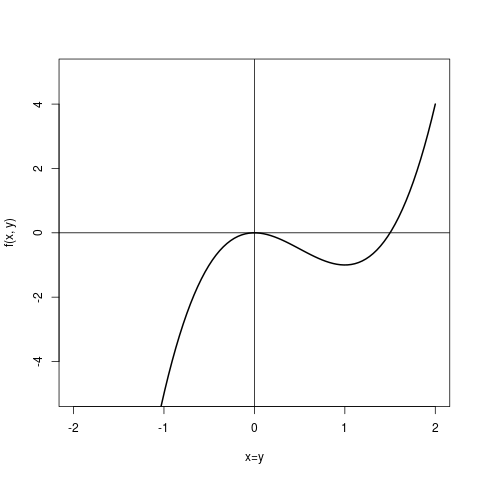
\includegraphics[width=.35\textwidth, trim=00 10 10 40, clip=]{ExempleOptimum-1ereBissectrice} &
        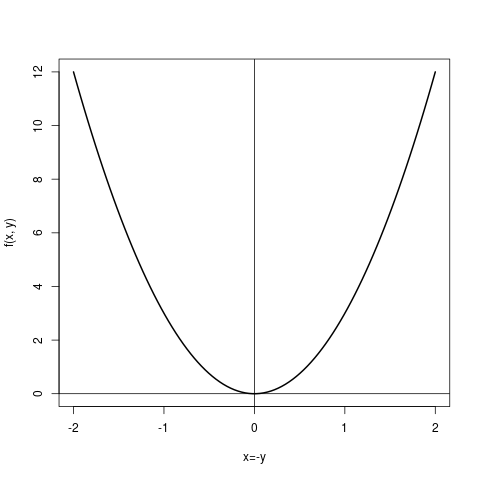
\includegraphics[width=.35\textwidth, trim=00 10 10 40, clip=]{ExempleOptimum-2emeBissectrice} \\
        $f(x, x) = 2x^3 - 3x^2$ & $f(x, -x) = 3x^2$
      \end{tabular}
      $$
      \item[\'Etude du point $b$ :] on a
      $$
      \nabla_b^2 f = \left[\begin{array}{rrr} 6 & & -3 \\ -3 & & 6 \end{array}\right]
      \qquad \Rightarrow \qquad 
      | \nabla_b^2 f | = 27 > 0, \qquad \tr(\nabla_b^2 f) = 12 > 0
      $$
      donc les deux valeurs propres de $\nabla_b^2 f$ sont positives : $b$ est donc un minimum.
    \end{description}
    Au total la surface d'équation $\{z = f(x, y)\}$ a l'aspect suivant
    $$
    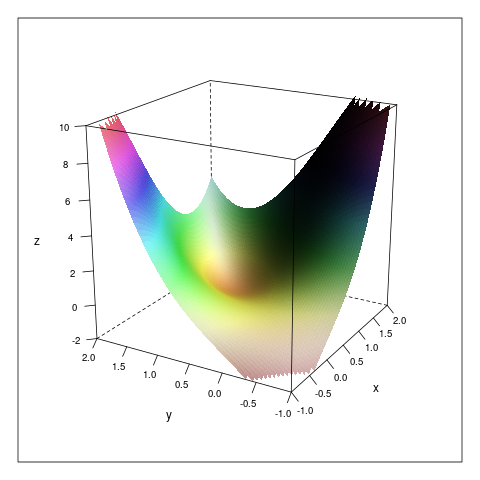
\includegraphics[width=.6\textwidth]{ExempleOptimum-surface}
    $$
  }
\end{enumerate}



% Voir \url{www.bibmath.net/ressources/index.php?action=affiche&quoi=bde/analyse/calculdiff/extrema&type=fexo}, exercice 7 (en fait, bof : un peu long)

Voir \url{www.bibmath.net/ressources/index.php?action=affiche&quoi=bde/analyse/calculdiff/extrema&type=fexo}, exercice 16


\newpage \section{\'Equations différentielles et systèmes dynamiques} \newcommand{\equadiff}{/home/robin/ENSEIGN/Cours/MathBiologie/L3-ENS-Math1/Exercices/EquaDiff}

%-------------------------------------------------------------------------------
\subsection{Calcul différentiel}
%-------------------------------------------------------------------------------

%-------------------------------------------------------------------------------
\subsubsection{Application linéaire tangente à une forme quadratique} 
%-------------------------------------------------------------------------------

On considère une matrice $A \in \Mcal_n$ symétrique, un vecteur $v \in \Rbb^n$ et la fonction 
$$
\begin{array}{rlll}
  f : & \Rbb^n & \mapsto & \Rbb \\
  & x & \to & f(x) = x^\top A x + v^\top x.
\end{array}
$$

\begin{enumerate}
  \item Montrer qu'il existe un vecteur $g(x) \in \Rbb^n$, qu'on précisera, tel que l'application linéaire tangente à $f$ en $x$ s'écrit
  $$
  \begin{array}{rlll}
    D_xf : & \Rbb^n & \mapsto & \Rbb^n \\
    & h & \to & D_xf(h) = g(x)^\top h.
  \end{array}
  $$
  \solution{On écrit
  \begin{align*}
    f(x+h) 
    & = (x+h)^\top A (x+h) + v^\top (x+h)
    = f(x) + x^\top A h + h^\top A x + h^\top A h + v^\top h \\
    & = f(x) + (2 x^\top A + v^\top) h + h^\top A h
  \end{align*}
  puisque $x^\top A h = h^\top A x$. On remarque alors que $h^\top A h = o(\|h\|)$ pour conclure que, puisque $A$ est symétrique, l'application linéaire tangent $D_x f$ s'écrit bien
  $$
  D_xf(h) = g(x)^\top h
  \qquad \text{avec} \quad
  g(x) = 2 A x + v.
  $$}
  \item En supposant que $A$ est inversible, déterminer le point stationnaire $x^*$ où $g(x)$ s'annule.
  \solution{En supposant $A$ inversible, on a
  $$
  g(x^*) = 0
  \qquad \Leftrightarrow \qquad
  2 A x^* + v = 0
  \qquad \Leftrightarrow \qquad
  x^* = - \frac12 A^{-1} v.
  $$}
  \item Donner une condition sur$A$ pour que $A$ soit un minimum local. (On pourra calculer la matrice hessienne de $A$.)
  \solution{La matrice hessienne de l'application $f$ en tout point $x$ vaut $H_x = 2 A$ (il suffit de déterminer l'application linéaire tangente à $g(x)$).
  $x^*$ est donc un minimum ssi $A$ est strictement définie négative}
  \item Discuter l'utilité de l'hypothèse selon laquelle $A$ est symétrique.
  \solution{On peut décomposer $A$ en ses parties symétrique $S$ et anti-symétrique $T$ : 
  $$
  S = \frac12(A + A^\top), \qquad 
  T = \frac12(A - A^\top), \qquad 
  \Rightarrow \quad
  A = S + T
  $$
  et remarquer que
  $$
  f(x) 
  = x^\top A x + v^\top x
  = x^\top S x + \frac12 \underset{=0}{\underbrace{(x^\top A x - x^\top A^\top x)}} + v^\top x,  
  $$
  c'est-à-dire que seulle la partie symétrique de $A$ contribue à la fonction Ode $f$.}
\end{enumerate}




%-------------------------------------------------------------------------------
\subsection{Systèmes dynamiques en dimension 1}
%-------------------------------------------------------------------------------

%-------------------------------------------------------------------------------
\subsubsection{L3 Bio SU : TD2, exercice 1 \todo{}} 
%-------------------------------------------------------------------------------

\todo{Voir L3 Bio SU : TD2, exercice 1}


%-------------------------------------------------------------------------------
\subsubsection{Système différentiel d'ordre trois} 
%-------------------------------------------------------------------------------

On considère l'équation différentielle ordinaire non-linéaire
\begin{equation} \label{eq:L3BioSUTD2E2}
\dot x = f(x) = -x^3 + 7x^2 - 14x + 8.
\end{equation}
% dans laquelle $x$ désigne la concentration d'un métabolite : \eqref{eq:L3BioSUTD2E2} modélisant l'ensemble des réactions biochimiques impliquées dans la production/dégradation de ce métabolite.

\begin{enumerate}
  \item Déterminer l'ensemble des points stationnaires de \eqref{eq:L3BioSUTD2E2}.
  \solution{On cherche les raçines de $f(x)$. 1 est une racine évidente, et, en déterminant les raçines de $x^2 - 6x + 8$, on voit que $f(x)$ se factorise en
  \begin{align*}
    f(x) & = (x-1) (x^2 - 6x + 8) = (x-1) (x - 2) (x - 4). 
  \end{align*}
  Les points stationnaires sont donc $x^*_1 = 1$, $x^*_2 = 2$ et $x^*_3 = 4$.}
  \item \'Etudier la stabilité de chacun de ces points stationnaires.
  \solution{On calcule
  $$
  f'(x) = -3 x^2 + 14x -15
  $$
  et on conclue 
  \begin{align*}
    f'(x^*_1) & = -3 < 0 & \Rightarrow \quad x^*_1 & = 1 \text{ est stable}, \\ 
    f'(x^*_2) & = + 2 > 0 & \Rightarrow \quad x^*_2 & = 2 \text{ est instable}, \\ 
    f'(x^*_3) & = -6 < 0 & \Rightarrow \quad x^*_3 & = 4 \text{ est stable}. 
  \end{align*}}
  \item Tracer le diagramme de stabilité du système.
  \solution{$$
  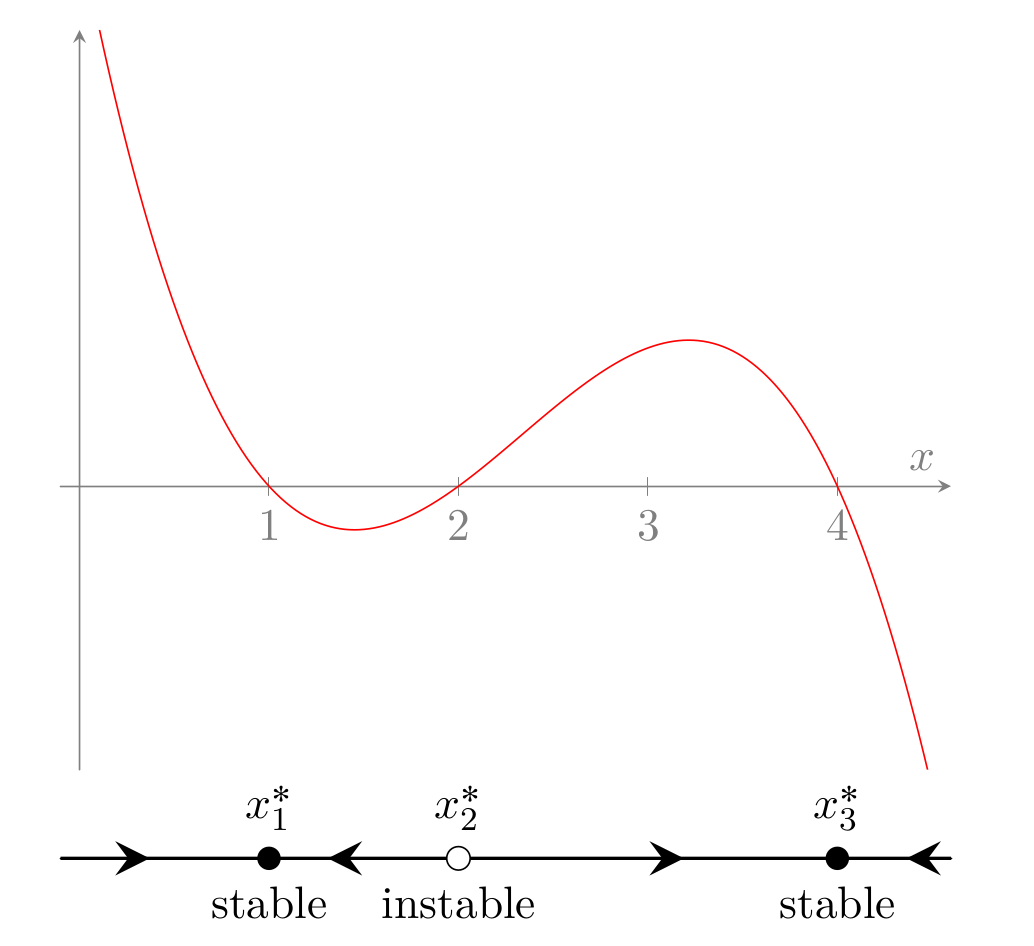
\includegraphics[width=.4\textwidth]{L3bioSU-TD2exo2}
  $$}
  \item D'un point de vue du comportement du système, quels sont les rôles respectifs de chacun des points stationnaires.
  \solution{
  \begin{itemize}
   \item $x^*_1$ et $x^*_3$ sont des équilibre stables et attracteurs vers lesquels le système tend. On perle de bistabilité.
   \item $x^*_2$ est le point critique (stationnaire mais répulsif) : la position de $x(0$ par rapport à $x^*_2$ détermine l'état final du système.
  \end{itemize}}
\end{enumerate}


%-------------------------------------------------------------------------------
\subsubsection{Modèle cubique}
%-------------------------------------------------------------------------------

% [Exercice 2, TD2, L2 Bio SU]

\exemple{
  On considère le système
  $$
  \dot y = - y^3 + 7 y^2 - 14 y + 8.
  $$
  Ses points stationnaires sont les racines du polynôme $P(y) = - y^3 + 7 y^2 - 14 y + 8$, donc $y_1 = 1$ fait partie, donc
  $$
  P(y) = (y-1) (-y^2 + 6y + 8),
  $$
  et les deux racines de $-y^2 + 6y + 8$ sont $2$ et $4$. Les points stationnaires du système sont donc 
  $$
  y_1 = 1, \qquad y_2 = 2, \qquad y_3 = 4.
  $$
  Leur stabilité est donné par la dérivée de $P$:
  $$
  P'(y) = -3y^2 + 14 y - 14,
  $$
  soit
  $$
  P'(y_1) = -3, \qquad P'(y_2) = 2, \qquad P'(y_3) = -6.
  $$
  $y_1$ et $y_3$ sont donc des équilibres stables, et $y_2$ un équilibre instable.
  $$
  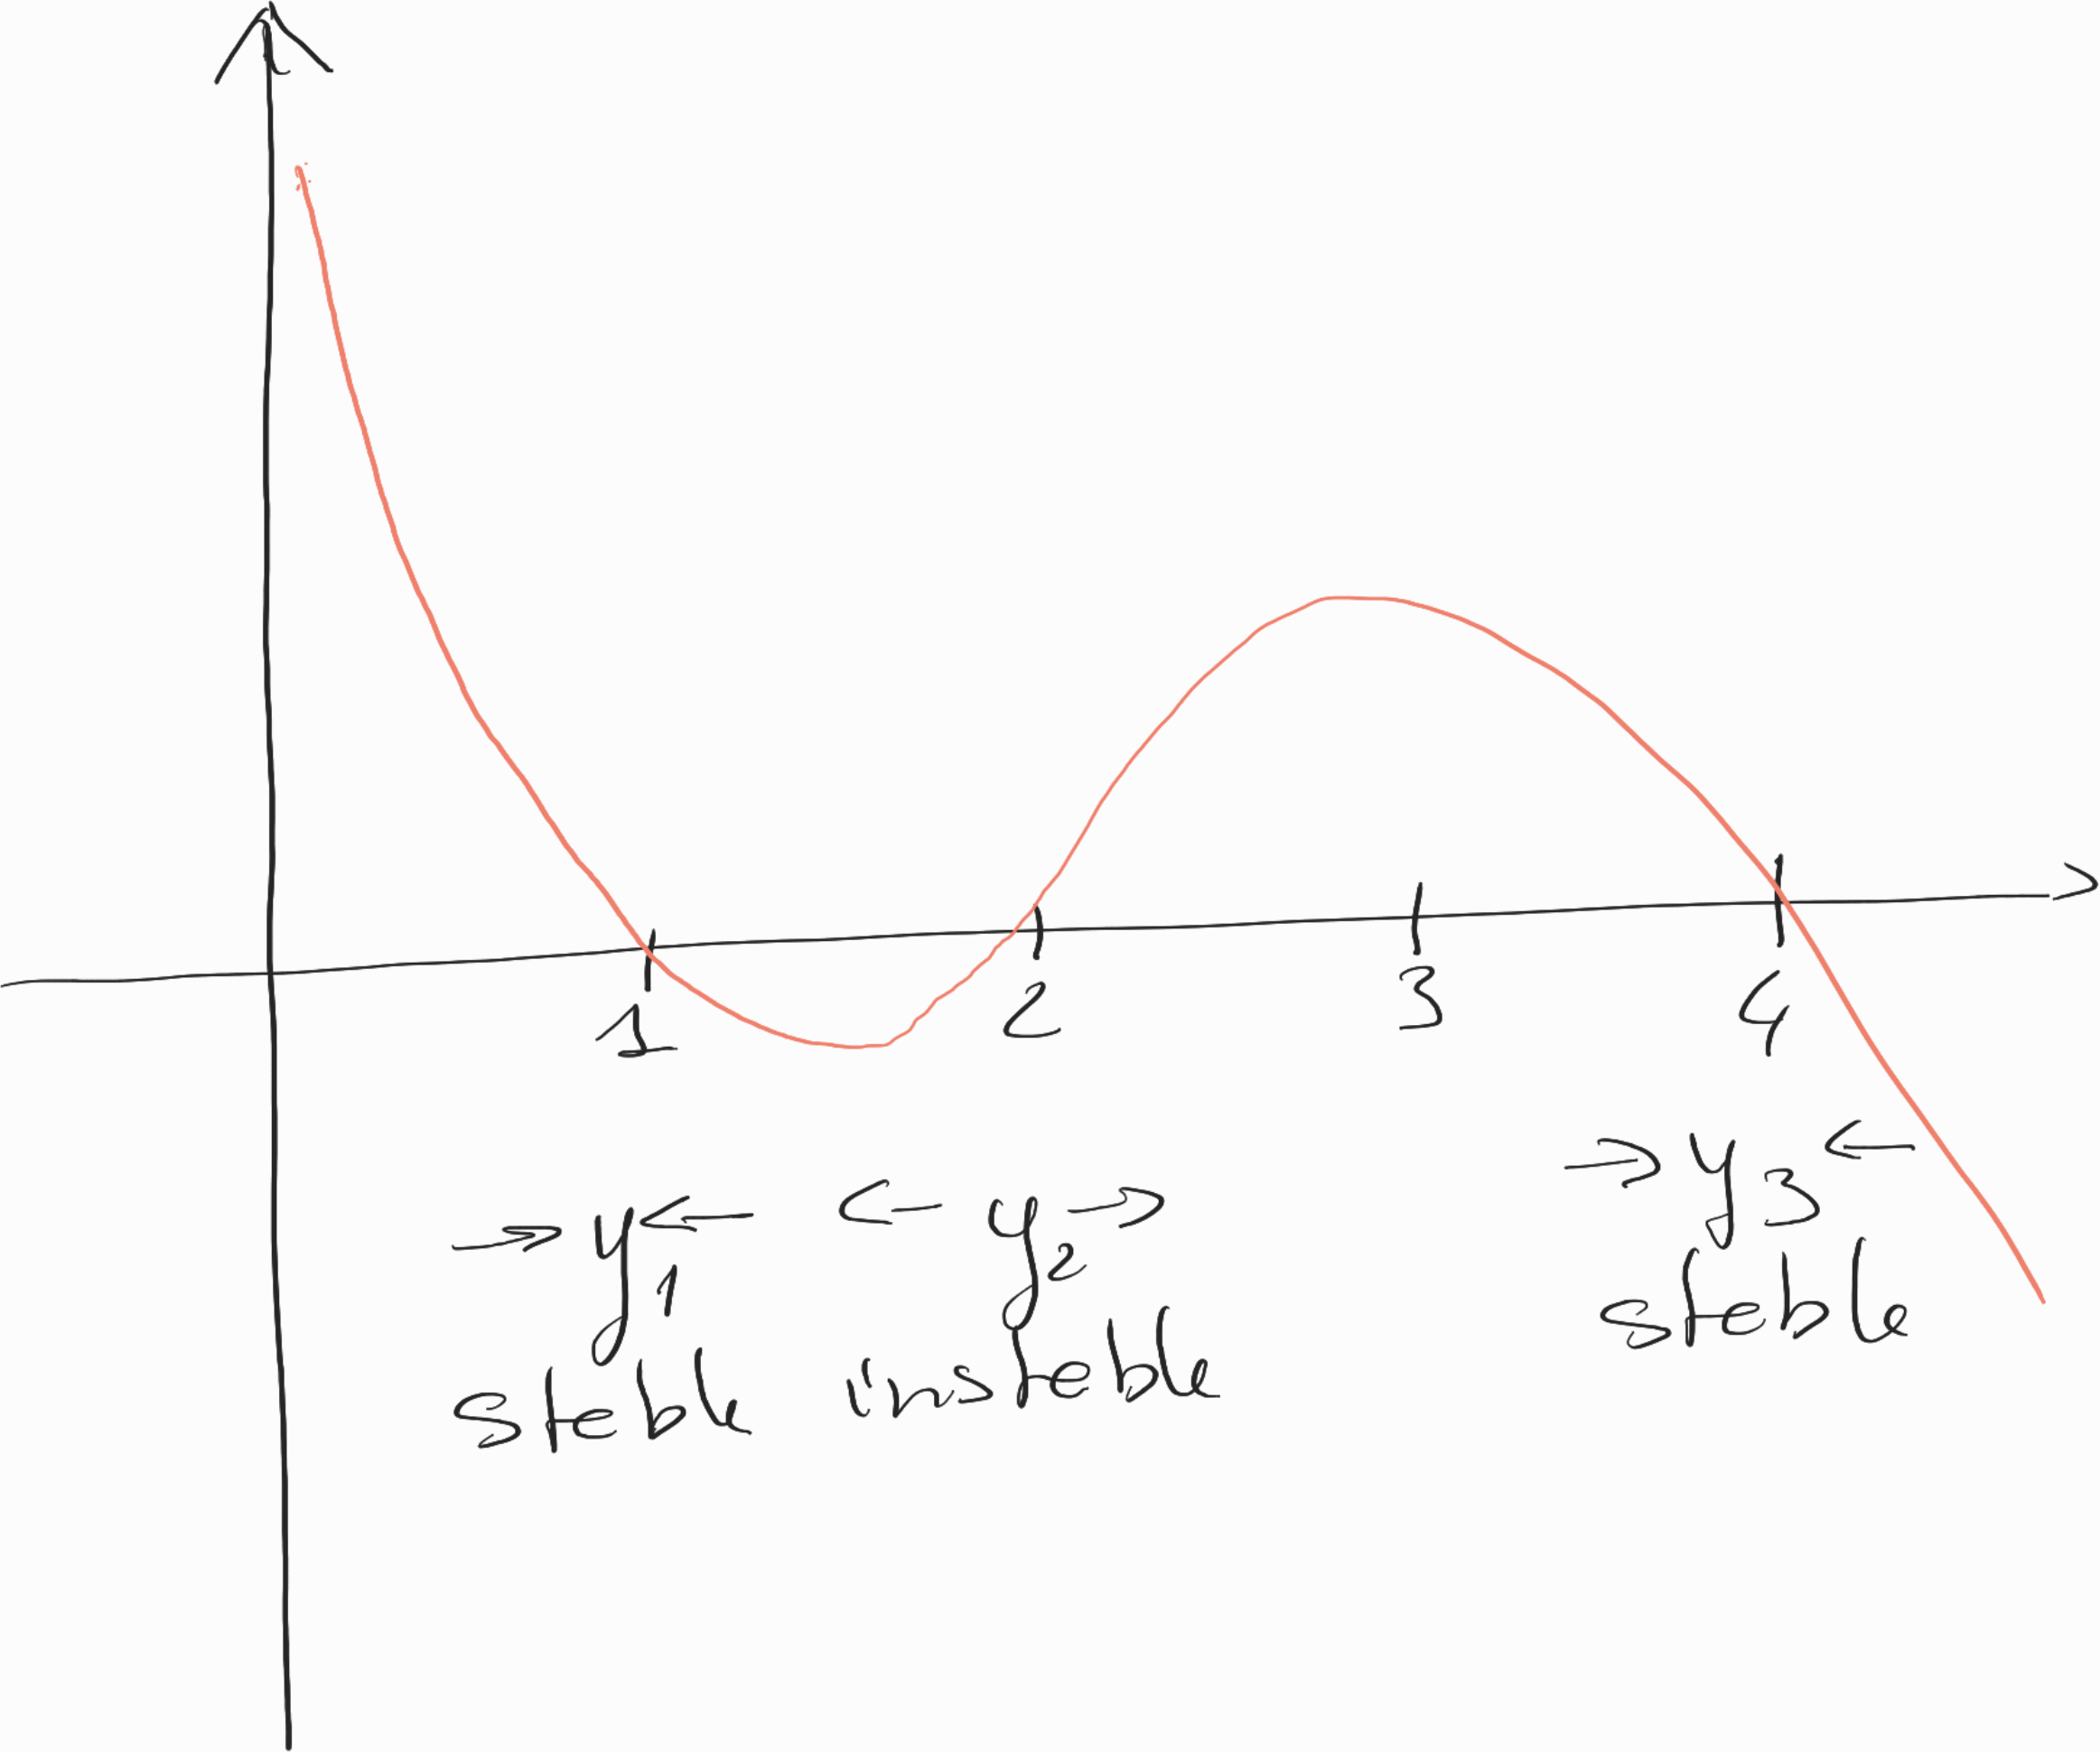
\includegraphics[width=.5\textwidth]{TD-SUbioL3-TD2Exo2}
  $$
}




%-------------------------------------------------------------------------------
\subsubsection{Système dynamique en $y^5$ \todo{}}
%-------------------------------------------------------------------------------

On souhaite déterminer les points d'équilibre (et leur nature) du système
$$
\dot y = F(y) = \mu y + 2 y^3 - y^5.
$$
On a 
$$
F(y) = y(\mu + y^2 - y^4)
$$
qui s'annule pour $y = 0$ et pour les solutions de $(\mu + 2 y^2 - y^4)$. En posant, $z = y^2$, $\mu + 2 z - z^2 = 0$ admet des solutions si $\Delta =  4(1 + \mu) \geq 0$, soit $\mu \geq -1$. Ces solutions sont alors $z^* = -1 \pm \sqrt{1+\mu}$. La seule solution possiblement positive est $z^* = -1 + \sqrt{1+\mu}$ et elle l'est ssi $\mu > 1$. \\
Le système admet donc un unique point fixe $x^*=0$ si $\mu < 1$ et un second point fixe $x^* = -1+\sqrt{1+\mu}$ si $\mu > 1$. \\
On a de plus
$$
F'(x) = \mu + 3 y^2 - 5y^4
$$
dont le signe est celui de $\mu$ pour $x=0$ et \todo{nature de $x^* = -1+\sqrt{1+\mu}$ si $\mu > 1$.}


%-------------------------------------------------------------------------------
\subsection{Systèmes dynamiques en dimension 2}
%-------------------------------------------------------------------------------

% \todo{Examen L3-Bio-SU 2022-23 : Exercice 2}

%-------------------------------------------------------------------------------
\subsubsection{Système dynamique linéaire.} 
%-------------------------------------------------------------------------------

On considère le système dynamique suivant
$$
\left\{\begin{array}{rcl}
        \dot x & = & -a_1 x + b_1 y + c_1 \\ 
        \dot y & = & -a_2 x + b_2 y + c_2
        \end{array}\right.
$$
où tous les coefficients constants sont strictement positifs.
\begin{enumerate}
  \item À quelle condition y a-t-il un unique équilibre ? Lorsque c’est le cas, à quelle condition est-il stable ?
  \solution{\todo{}}
  \item Lorsqu’il n’existe pas d’équilibre unique, représenter les deux isoclines (c'est à dire les ensemble de points ou s'annule $\dot x$ d'une part et $\dot y$ d'autre part). Y a-t-il une infinité d’équilibres ou aucun équilibre ?
  \solution{\todo{}}
  \item Représenter les orbites dans le plan de phase.
  \solution{\todo{}}
\end{enumerate}


%-------------------------------------------------------------------------------
\subsubsection{Système dynamique quadratique} \label{SystDyn-Quadratique}
%-------------------------------------------------------------------------------

On considère le système dynamique d’activation réciproque avec compétition intraspécifique suivant 
$$
%   \SR{
%   \left\{\begin{array}{rcl}
%          \dot x & = & r y - cx^2 \\ 
%          \dot y & = & r x - cy^2 
%          \end{array}\right.
%   }{
\left\{\begin{array}{rcl}
        \dot x & = & a y - x^2 \\ 
        \dot y & = & a x - y^2 
        \end{array}\right.
%   }
$$
%   où $r$ et $c$ sont deux constantes strictement positives.
où $a$ est une constante strictement positive.
\begin{enumerate}
  \item Déterminer les équilibres de ce modèle.
  \solution{$(x=0, y=0)$ est un point d'équilibre trivial. L'autre point d'équilibre s'obtient en résolvant
  $$
  \left\{\begin{array}{rcl}
          a y & = & x^2 \\
          a x & = & y^2
        \end{array}\right.
  \quad \Leftrightarrow \quad
  \left\{\begin{array}{rcl}
          y & = & x^2 / a \\
          a x & = & x^4 / a^2
        \end{array}\right.
  \quad \Leftrightarrow \quad
  \left\{\begin{array}{rcl}
          y & = & x^2 / a \\
          a^3 & = & x^3
        \end{array}\right.
  \quad \Leftrightarrow \quad
  x^* = y^* = a.
  $$}
  \item Donner la nature de chacun de ces deux équilibres.
  \solution{En notant
  $$
  F(x, y) = \left[\begin{array}{rcl} 
                    F_1(x, y) & = & ay - x^2 \\
                    F_2(x, y) & = & ax - y^2
                  \end{array}\right],
  $$
  on a
  $$
  J_{(x, y)} F = \left[\begin{array}{cc}-2x & a \\ a & -2y\end{array}\right].
  $$
  \begin{description}
    \item[Point $(0, 0)$:] on a
    $$
    J_{(0, 0)} F = \left[\begin{array}{cc}0 & a \\ a & 0\end{array}\right]
    \quad \Rightarrow \quad
    P(\lambda) = \lambda^2 - a^2
    $$
    qui s'annule pour $\lambda = \pm a$. Des vecteurs associés à $a$ et $-a$ sont, respectivement $[1 \; 1]^\top$ et $[-1 \; 1]^\top$. \\
    $(0, 0)$ est un équilibre instable dans la direction de la première bissectrice et stable dans celle de la seconde.
    \item[Point $(a, a)$:] on a
    $$
    J_{(0, 0)} F = \left[\begin{array}{cc}-2a & a \\ a & -2a\end{array}\right]
    \quad \Rightarrow \quad
    P(\lambda) = \lambda^2 - a^2
    \quad \Rightarrow \quad
    P(\lambda) = \lambda^2 - 4 a \lambda + 3 a^2
    $$
    qui s'annule pour $\lambda = -a$ et $\lambda = -3a $. \\
    $(a, a)$ est donc un équilibre stable.
  \end{description}
  }
  \item Que se passe-t-il si $x(0) = y(0) > 0$ ? Représenter l’allure des trajectoires dans le plan de phase. 
  \solution{
  On peut remarquer que 
  $$
  \dot x \geq 0 \quad \Leftrightarrow \quad y \geq x^2/a, \qquad \qquad
  \dot y \geq 0 \quad \Leftrightarrow \quad y \leq \sqrt{a x}.
  $$
  $$
  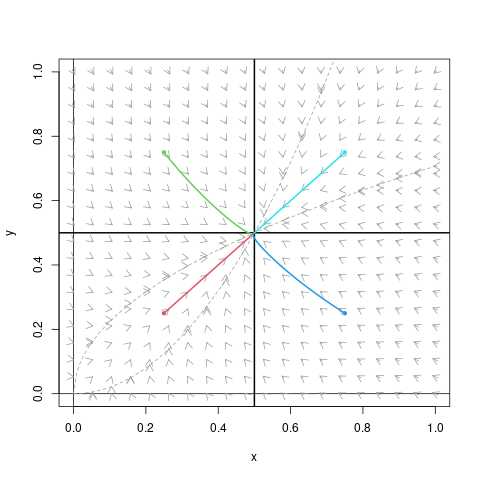
\includegraphics[width=.45\textwidth, trim=0 10 20 20, clip=]{ActivationReciproque}
  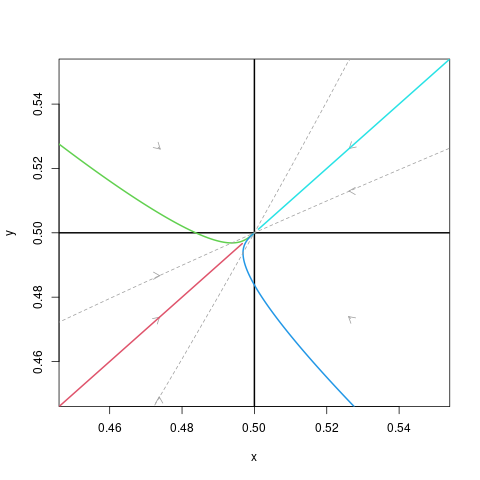
\includegraphics[width=.45\textwidth, trim=0 10 20 20, clip=]{ActivationReciproque-zoom}
  $$
  Toutes les trajectoires convergent vers $(a, a)$.
  \begin{description}
    \item[$(x_0 < a, y_0 < a)$:] la trajectoire converge directement vers $(a, a)$.
    \item[$(x_0 < a, y_0 > a)$:] la trajectoire franchit l'axe $y = a$ avant de revenir en $(a, a)$.
    \item[$(x_0 > a, y_0 > a)$:] la trajectoire converge directement vers $(a, a)$.
    \item[$(x_0 > a, y_0 < a)$:] la trajectoire franchit l'axe $x = a$ avant de revenir en $(a, a)$.
  \end{description}
  }
\end{enumerate}



%-------------------------------------------------------------------------------
\subsubsection{Système proie prédateur} 
%-------------------------------------------------------------------------------

On considère le système proie-prédateur suivant
\begin{equation} \label{eq:L3bioProiePredateur}
\left\{\begin{array}{rcl}
        \dot x & = & \displaystyle{x \left(1 - \frac{x}2\right) - \frac{xy}{1+x}} \\
        \dot y & = & \displaystyle{\frac{x-1}{x+1} y}
       \end{array}\right..
\end{equation}
% dans laquelle $x$ désigne la concentration d'un métabolite : \eqref{eq:L3BioSUTD2E2} modélisant l'ensemble des réactions biochimiques impliquées dans la production/dégradation de ce métabolite.

\begin{enumerate}
\item Qui sont les proies, qui sont les prédateurs ?
  \solution{$x =$ proies, $y = $ prédateurs : 
    \begin{itemize}
    \item Le terme d'interaction $xy$ intervient avec un signe négatif dans le taux de croissance $\dot x$, ce qui est caratéristique du comportement d'une population de proies confrontées à des prédateurs.
    \item Pour $x=0$, on obtient $\dot y = -y$ qui décrit un comportement d'une population de prédateurs qui s'éteint en l'absence de proie. 
    \end{itemize}}
\item Déterminer les points stationnaires du systèmes.
  \solution{En distinguant les cas $y = 0$ et $y \neq 0$, on vérifie facilement que
  $$
  m^*_1 = \left(\begin{array}{c}0 \\ 0\end{array}\right), \qquad
  m^*_2 = \left(\begin{array}{c}2 \\ 0\end{array}\right), \qquad
  m^*_3 = \left(\begin{array}{c}1 \\ 1\end{array}\right)
  $$
  sont les seuls points stationnaires.}
\item Montrer que $y=0$ est une solution du système. Quel est le comportement de $x$ dans ce cas ?
  \solution{$y \equiv 0$ satisfait la seconde équation du système. La première équation devient alors $\dot x = x \left(1 - x/2\right)$ : la population des proies évolue selon un modèle logistique.}
\item Déterminer la matrice jacobienne $J_{x, y}$ du système
  \solution{On a
  $$
  J_{x, y} = \left[\begin{array}{ccc}
                   \displaystyle{(1 - x) - \frac{y}{(1+x)^2}} & & 
                   \displaystyle{\frac{-x}{1+x}} \\
                   \displaystyle{\frac{2 y}{(x+1)^2}} & & 
                   \displaystyle{\frac{x-1}{x+1}}
                  \end{array}\right]
  $$}
  \item \'Etudier la stabilité des points stationnaires.
  \solution{
  \begin{description}
  \item[$m^*_1 = (0, 0) : $] on a 
    $$
    J_{m^*_1} = \left[\begin{array}{ccc}
                    {1} & & 
                    {0} \\
                    {0} & & 
                    {-1/2}
                    \end{array}\right]
    $$
    dont les valeurs propres sont 1 (associée à $u = (1, 0)$) et $-1/2$ (associée à $u = (0, 1)$). \\
    Il s'agit donc d'un point selle : l'équilibre est instable. Plus précisément, il est instable dans la direction de l'axe des $x$ (en l'absence de prédateur, la population de proies croît) et stable dans la direction de l'axe des $y$ (en l'absence de proie, les prédateurs s'éteignent).
  \item[$m^*_2 = (0, 0) : $] on a 
    $$
    J_{m^*_2} = \left[\begin{array}{ccc}
                    {-1} & & 
                    {-2/3} \\
                    {0} & & 
                    {1/3}
                    \end{array}\right]
    $$
    qui est triangulaire : ses valeurs propres sont $-1$ (associée à $u = (1, 0)$) et $1/3$ (associée à $u = (0, 1)$). \\
    Il s'agit aussi d'un point selle : l'équilibre est donc instable. Plus précisément, il est stable dans la direction de l'axe des $x$ (en l'absence de prédateur, la population de proies tend vers 2) et instable dans la direction de l'axe des $y$ (pour $x=2$, la population des prédateurs croît).
  \item[$m^*_3 = (1, 1) : $] on a 
    $$
    J_{m^*_3} = \left[\begin{array}{ccc}
                    {-1/4} & & 
                    {-1/2} \\
                    {1/2} & & 
                    {0}
                    \end{array}\right]
    $$
    dont le polynôme caractéristique est $P(\lambda) = \lambda^2 + \lambda/4 + 1/4.
    $. Son discriminant est $\Delta = 1/16 - 1 = -15/16$ : les valeurs propres sont donc $\lambda_1 = (-1 + i\sqrt{15})/8$ et $\lambda_2 = (-1 -\sqrt{15})/8$. \\
    Les parties réelles des valeurs propres sont négatives, donc l'équilibre est stable.
  \end{description}}
  \item Tracer le comportement du système aux abords de chacun des points stationnaires.
  \solution{Quelques exemples de trajectoires
  $$
  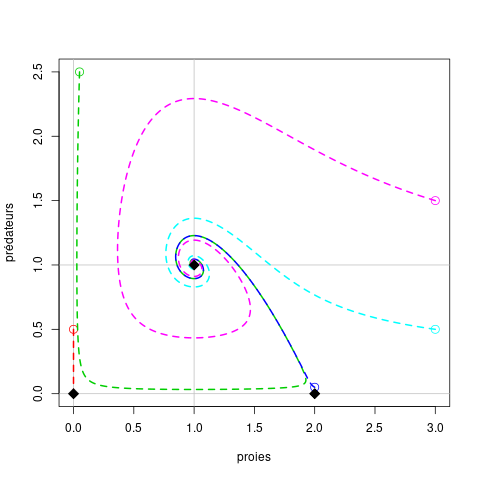
\includegraphics[width=.5\textwidth, trim=0 0 30 60, clip=]{L3bioSU-ProiePredateur-paths}
  $$
  $$
  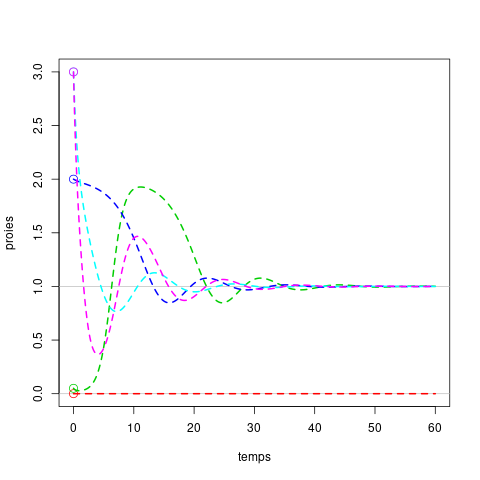
\includegraphics[width=.45\textwidth, trim=0 0 30 60, clip=]{L3bioSU-ProiePredateur-proies}
  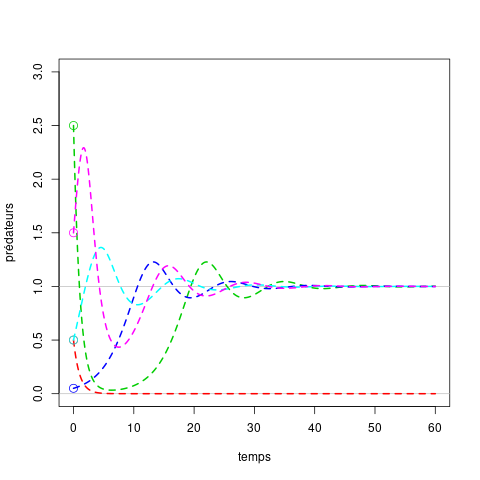
\includegraphics[width=.45\textwidth, trim=0 0 30 60, clip=]{L3bioSU-ProiePredateur-predateurs}
  $$
  }
\end{enumerate}


% Cycle limite \todo{Voir exemple 1, p 195, Perko, 2001}

%-------------------------------------------------------------------------------
\subsubsection{Modèle de Lotka-Volterra avec densité dépendance} 
%-------------------------------------------------------------------------------

\paragraph{Rappel.}
En notant 
\begin{itemize}
  \item $x(t)$ une variable proportionnelle au nombre de proies et
  \item $y(t)$ une variable proportionnelle au nombre de prédateurs,
\end{itemize}
le modèle Lotka-Volterra classique s'écrit, 
\begin{equation} \label{eq:LV}
\left\{\begin{array}{rcr}
        \dot x & = & r x (1 - y), \\ 
        \dot y & = & - m y (1 - x).
        \end{array}\right.
\end{equation}
Notamment, ce modèle admet deux points d'équilibre en $(x=0, y=0)$ et $(x=1, y=1)$.

\paragraph{Prise en compte d'une densité-dépendance.}
On considère ici un modèle de Lotka-Volterra avec densité dépendance. Plus précisément, en supposant le taux de croissance des proies égale à 1 ($r = 1$), on pose le modèle
\begin{equation} \label{eq:LVDD}
\left\{\begin{array}{rcr}
        \dot x & = & x (1 - y - ax), \\ 
        \dot y & = & - m y (1 - x), 
        \end{array}\right.
\end{equation}
où les paramètres $m$ et $a$ sont strictement positifs. 
% On remarque que le cas $a=0$ correspond au modèle de Lotka-Volterra classique (avec $r=1$).

\bigskip
\paragraph{Interprétation du modèle \eqref{eq:LVDD}.}
\begin{enumerate}
  \item Interpréter les paramètres $m$ et $a$ du modèle \eqref{eq:LVDD}.
  \solution{$m$ est le taux de mort des prédateurs en absence de proies (si $x(0)= 0$, $y(t) = y_0 e^{-mt}$). $a$ rend compte de la compétition entre les proies, c'est-à-dire de la limitation des ressources du milieu.}
  \item Déterminer les points d'équilibre du système \eqref{eq:LVDD}.
  \solution{
  L'isocline $\{\dot x = 0\}$ est $\Ical_x = \{x = 0\} \cup \{y = 1 - ax\}$ et l'isocline $\{\dot y = 0\}$ est $\Ical_y = \{y = 0\} \cup \{x = 1\}$. Les points d'équilibre sont donc $(0, 0)$, $(0, 1/a)$ et $(1, 1-a)$.}
  \item Expliquer la position du point d'équilibre $(x^*, y^*)$ non nul (c'est-à-dire pour lequel $x^*$ et $y^*$ sont non nuls) par rapport au point d'équilibre non nul du modèle de Lotka-Volterra classique \eqref{eq:LV}.
  \solution{L'équilibre non-trivial du modèle de Lotka-Volterra est le point $(1, 1)$. Le point d'équilibre des proies est conservé ($x^* = 1$), mais celui des prédateurs diminue $y^* = 1-a < 1$ : la contrainte imposée par le milieu au proies nuit, {\it in fine} à la population des prédateurs.}
\end{enumerate}

\bigskip
\paragraph{Questions intermédiaires (I).}
Soit la fonction $f: \Rbb^{*+} \mapsto \Rbb$, définie par $f(x) = \sqrt{x(x+1)} - x$.
\begin{enumerate}
  \setcounter{enumi}{3}
  \item Montrer que $f(x) > 0$. \label{q:LVDD-f1}
  \solution{On a $\sqrt{x(x+1)} > \sqrt{x^2} = x$, donc $f(x) > 0$.
  }
  \item Montrer que $f(x) < 1/2$. \label{q:LVDD-f2}
  \solution{On a
  $$
  f(x) < \frac12 
  \qquad \Leftrightarrow \qquad
  x(x+1) < \left(x + \frac12\right)^2
  \qquad \Leftrightarrow \qquad
  x^2 + x < x^2 + x + \frac14
  $$
  qui est toujours vrai.
  }
\end{enumerate}

\bigskip 
\paragraph{Questions intermédiaires (II).}
Soit la matrice $J^*$ définie par
\begin{equation} \label{eq:LVDD-Jstar}
  J^* = \left(\begin{array}{cc}
              -a & -1 \\ m(1-a) & 0
              \end{array}\right).
\end{equation}

\bigskip
\begin{enumerate}
  \setcounter{enumi}{5}
  \item Déterminer le polynôme caractéristique $P$ de $J^*$.
  \solution{$P(\lambda) = \lambda^2 + a \lambda + m(1-a)$.}
  %
  \item Montrer que les valeurs propres de $J^*$ sont réelles si et seulement si $a \geq a_1 = 2 f(m)$, où $f$ est la fonction définie en (I). 
  ({\sl On pourra étudier le discriminant $\Delta$ de $P$ comme une fonction de $a$.})
  \solution{La nature des valeurs propres de $J^*$ est donnée par le signe du discriminant de $P$ : $\Delta = \Delta(a) = a^2 + 4am - 4m$ qui est lui même un polynôme en $a$. \\
  Son discriminant est $\delta = 16m^2 + 16m = 16 m(m+1)$ est positif puisque $m$ est positif. 
  $\Delta(a)$ admet donc deux racines réelles:  $-2 (m + \sqrt{m(m+1)})$, qui est négative, et $a_1 = 2 (\sqrt{m(m+1)} - m) = 2f(m)$ qui est strictement positive d'après la question \ref{q:LVDD-f1}. 
  \\ $\Delta(a)$ est donc positif dès que $a \geq a_1 = 2 f(m)$ et $P$ admet alors deux racines réelles (égales si $a = a_1$). 
  }
  %
  \item Montrer que $a_1 < 1$ et que si $a > 1$, les valeurs propres de $J^*$ sont de signes différents. \label{q:racinePstar}
  \solution{
  La question \ref{q:LVDD-f2} nous assure que $a_1 = 2 f(m) < 1$, puisque $f(x) < 1/2$ pour tout $x \geq 0$. \\
  Si $a > a_1$, $P$ admet pour racines réelles $\lambda_1 = -(a +\sqrt{\Delta(a)})/2$, qui est toujours négative, et $\lambda_2 = (-a + \sqrt{\Delta(a)})/2$, qui est est positive dès que 
  $$
  \sqrt{\Delta(a)} \geq a
  \qquad \Leftrightarrow \qquad
  a^2 + 4am - 4m \geq a^2
  \qquad \Leftrightarrow \qquad
  a \geq 1.
  $$
  $J^*$ a donc des valeurs propres de racines distinctes dès que $a > 1 > a_1$. \\ 
  Alternativement, par les propriétés du polynôme caractéristique d'une matrice de $\Mcal_2$, $\lambda_1$ et $\lambda_2$ sont de même signe ssi $\lambda_1 \lambda_2 = |J^*| = m(1-a) > 0$, c'est-à-dire si $a <1$, puisque $m > 0$.
  }
\end{enumerate}
  

\bigskip
\paragraph{Stabilité du point d'équilibre non nul.}
On s'intéresse maintenant à la stabilité du point d'équilibre $(x^*, y^*)$ non nul. 
\begin{enumerate}
  \setcounter{enumi}{8}
  \item Déterminer la matrice jacobienne du système en un point $(x, y)$ quelconque.
  \solution{
  $$
  J = \left(\begin{array}{cc}
            -2ax + (1-y) & -x \\ my & m(x-1) 
            \end{array}\right).
  $$
  }
  \item En déduire que la matrice jacobienne en $(x^*, y^*)$ est égale à la matrice $J^*$ définie à l'équation \eqref{eq:LVDD-Jstar}.
  \solution{Direct.}
  \item \'Etudier la nature de l'équilibre $(x^*, y^*)$ en fonction de la position de $a$ par rapport aux deux valeurs seuils $a_1$ et $1$ : $a < a_1$, $a_1 < a < 1$ ou $a > 1$.
  ({\sl On ne s'attardera pas sur les cas limites $a = a_1$ et $a = 1$}.)
  \solution{
  \begin{description}
    \item[$a < a_1$ :] dans ce cas, $\Delta(a) < 0$ et les valeurs propres de $J*$ sont $\lambda_1$ et $\lambda_2$ calculées à la question \ref{q:racinePstar}, qui sont complexes mais dont les parties réelles sont négatives puisque $a > 0$. L'équilibre $(x^*, y^*)$ est donc un équilibre stable.
    \item[$a_1 < a < 1$ :] dans ce cas, $\Delta(a) > 0$ et les valeurs propres $\lambda_1$ et $\lambda_2$ sont toutes les deux réelles et négatives : l'équilibre $(x^*, y^*)$ est donc toujours stable.
    \item[$a > 1$ :] $\lambda_1$ est toujours négative mais $\lambda_2$ devient positive et $(x^*, y^*)$ devient alors instable.
  \end{description}
  Les figures suivantes donnent respectivement les parties réelles $Re(\lambda)$ et imaginaires $Im(\lambda)$  des valeurs propres $\lambda_1$ et $\lambda_2$ en fonction de $a$ pour $m=1/2$. 
  $$
  \begin{array}{c}
    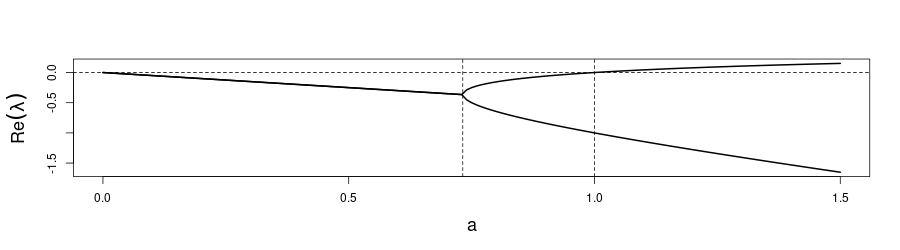
\includegraphics[width=.8\textwidth, trim=0 0 0 50, clip=]{LotkaVolterraDD-m0.5-eigenValueReal.png} \\
    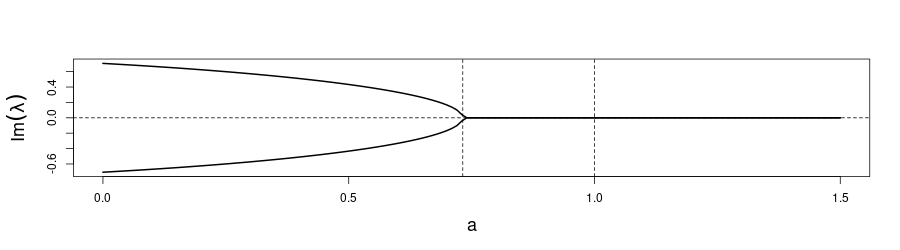
\includegraphics[width=.8\textwidth, trim=0 0 0 50, clip=]{LotkaVolterraDD-m0.5-eigenValueImaginary.png} 
  \end{array}
  $$
  La bifurcation se produit en $a = a_1$ et l'une des valeurs propres devient positive pour $a = 1$.
  }
\end{enumerate}

\bigskip
\paragraph{Trajectoires.}
Les trajectoires ($i$), ($ii$) et ($iii$) suivantes ont été obtenues par intégration numérique avec $m = 1/2$ et partant de l'état initial $(x_0 = 2,\;  y_0 = 3/2)$ pour trois valeurs de $a$ différentes :
$$
\begin{array}{ccc}
  (i) & (ii) & (iii) \\
  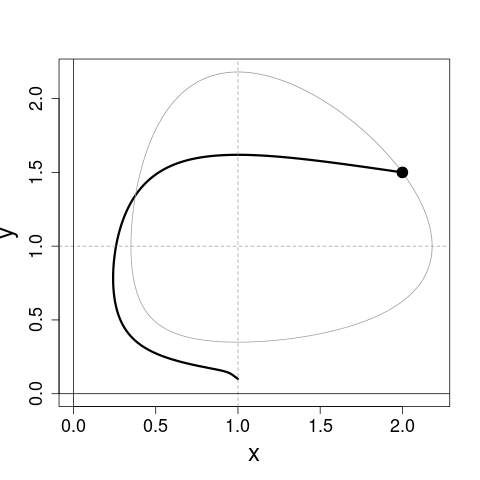
\includegraphics[width=.32\textwidth, trim=0 0 0 50, clip=]{LotkaVolterraDD-m0.5-a0.9.png} &
  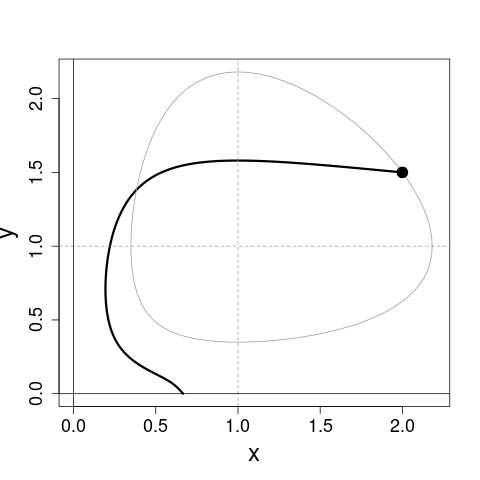
\includegraphics[width=.32\textwidth, trim=0 0 0 50, clip=]{LotkaVolterraDD-m0.5-a1.5.png} &
  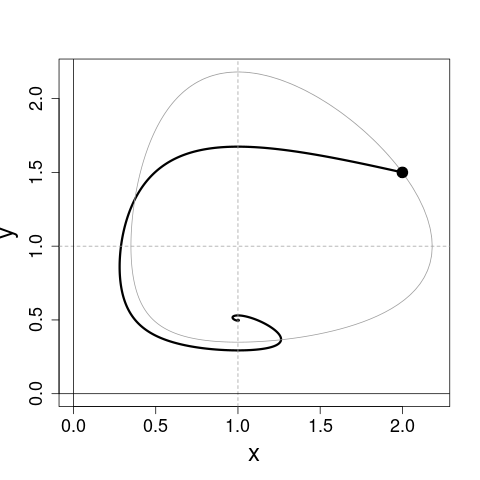
\includegraphics[width=.32\textwidth, trim=0 0 0 50, clip=]{LotkaVolterraDD-m0.5-a0.5.png}
\end{array}
$$
La courbe grise indique la trajectoire du modèle de Lotka-Volterra \eqref{eq:LV} sans densité-dépendance ($m = 1/2$, $a = 0$), partant du même point initial. Les repères grisés indiquent le point d'équilibre de ce même modèle \eqref{eq:LV}.

\begin{enumerate}
  \setcounter{enumi}{11}
  \item Associer chacune des trajectoires ($i$), ($ii$) et ($iii$) à l'une des trois valeurs de $a$ : $a = 1/2$, $a = 9/10$ et $a = 3/2$.
  \solution{On a dans ce cas $a_1 = 2 f(1/2) = \sqrt{3} - 1 \simeq 0.73$.
  \begin{description}
    \item[$a = 1/2 < a_1$ :] le système possède un équilibre stable en ($x^* = 1, y^* = 1/2$) et les valeurs propres de $J^*$ possèdent une partie imaginaire non nulle qui induit un enroulement autour de l'équilibre : on reconnaît la trajectoire ($iii$).
    \item[$a_1 < a = 9/10 < 1$ :] le système possède un équilibre stable en ($x^* = 1, y^* = 1/10$) mais les valeurs propres de $J^*$ sont réelles et négatives : le système tend vers l'équilibre sans enroulement : on reconnaît la trajectoire ($i$).
    \item[$a = 3/2 > a_1$ :] le système possède un équilibre instable en ($x^* = 1, y^* = -1/2$) que le système n'atteint jamais, du fait de l'extinction des prédateurs ($y(t) \to 0$) : on reconnaît la trajectoire ($ii$).
  \end{description}
  }
  \item Donner la limite de $x(t)$ quand $t$ tend vers l'infini dans le cas ($ii$).
  \solution{
  Dans ce cas, $y(t)$ tend vers 0 quand $t \to\infty$, le système \eqref{eq:LVDD-Jstar} devient donc simplement $\dot x = F(x)$ avec $F(x) = x (1 - ax)$. Ce système admet deux points d'équilibre en $x_1 = 0$ et $x_2 = 1/a$ et seul le second est stable (car $F'(x_1) > 0$ et $F'(x_2) < 0$). \\
  Après extinction des prédateurs, la population des proies tend donc vers un des équilibres 'nuls' : $(x_2 = 1/a = 2/3, y=0)$. Du fait de la densité-dépendance, la population des proies n'explose donc pas, contrairement au modèle de Lotka-Volterra classique.
  }
\end{enumerate}


%-------------------------------------------------------------------------------
\subsection{Dynamique des populations}
%-------------------------------------------------------------------------------

%-------------------------------------------------------------------------------
\subsubsection{Dynamique de population à trois classes : mâles, femelles et couples}
%-------------------------------------------------------------------------------

On considère une population sexuée panmictique, au sein de laquelle on désigne
respectivement par $x(t)$, $y(t)$ et $z(t)$ les densités au temps $t$ de femelles flottantes, de mâles flottants, et de couples. On suppose que la dynamique de la population respecte le système dynamique suivant
\begin{equation} \label{eq:Dyn3Pop}
  \left\{\begin{array}{rcl}
          \dot x(t) & = & - \alpha x y + r z, \\
          \dot y(t) & = & - \alpha x y + r z, \\
          \dot z(t) & = & + \alpha x y - c z^2,
          \end{array} \right.
\end{equation}
où les coefficients $\alpha$, $r$ et $c$ sont strictement positifs.
\begin{enumerate}
  \item Interpréter ces équations et la signification de chacun des coefficients $\alpha$, $r$ et $c$.
  \solution{Les mâles et femelles flottant(e)s s'apparient pour former des couples : 
  \begin{itemize}
    \item $\alpha$ est le taux de formation des couples, 
    \item $r$ est le taux de natalités de mâles et des femelles (supposés égaux),
    \item $c$ est le taux de mortalité des couples.
  \end{itemize}
  }
  \item En notant $S = x(0) - y(0)$, montrer que $x(t) - y(t) = S$ pour tout temps $t$. En
  déduire les fonctions $y$ et $z$ satisfont le système 
  \begin{equation} \label{eq:Dyn3Pop2}
    \left\{\begin{array}{rcl}
            \dot y(t) & = & - \alpha (y^2 + Sy) + r z, \\
            \dot z(t) & = & + \alpha (y^2 + Sy) - c z^2.
            \end{array} \right.
  \end{equation}
  Dans la suite on supposera que $S > 0$.
  \solution{On remarque que
  $$
  \dot x(t) - \dot y(t) = 0,
  $$
  ce qui implique que la différence $x(t) - y(t)$ reste constante au cours du temps et égale à $x(0) - y(0) = S$. \\
  On peut donc remplacer $x(t) = y(t) + S$ dans le système \eqref{eq:Dyn3Pop} pour obtenir le système \eqref{eq:Dyn3Pop2}.}
  \item Déterminer les points d'équilibre du système \eqref{eq:Dyn3Pop2}.
  \solution{
  \begin{itemize}
    \item $(y^* = 0, z^* = 0)$ est un équilibre (trivial).
    \item $(y = -S, z^* = 0)$ n'est pas un équilibre intéressant du point de vue du modèle car on s'intéresse aux effectifs positifs ou nuls. 
    \item Si on suppose $({y^*}^2 + Sy^*) \neq 0$, il vient
    $$
    \alpha({y^*}^2 + Sy^*) = rz^* = c{z^*}^2 
    \qquad \Rightarrow \qquad 
    z^* = r / c
    $$
    et $y^*$ doit vérifier
    $$
    {y^*}^2 + Sy^* - \frac{r^2}{\alpha c} = 0,
    $$
    dont le discriminant est 
    $$
    \Delta =  S^2 + \frac{4 r^2}{\alpha c} > S^2,
    $$
    et dont la seule solution positive est
    $$
    y^* = \frac{\sqrt{\Delta} - S}2.
    $$
    Le second équilibre intéressant est donc $(y^* = (\sqrt{\Delta} - S)/2, z^* = r/c)$. \\
    $(y^* = (-\sqrt{\Delta} - S)/2, z^* = r/c)$ est bien un point d'équilibre, mais sans intérêt du point de vue du modèle.
  \end{itemize}
  }
  \item \'Ecrire la matrice jacobienne du système \eqref{eq:Dyn3Pop2} et étudier la nature du ou des équilibres non triviaux.
  \solution{La jacobienne vaut
  $$
  J = \left[\begin{array}{rr}
              -2 \alpha y - \alpha S & r \\ 2 \alpha y + \alpha S & -2 c z
            \end{array}\right]
  $$
  \begin{description}
    \item[En $(0, 0)$ :] on a 
    $$
    J_{(0, 0)} = \left[\begin{array}{rr}
                - \alpha S & r \\ \alpha S & 0
              \end{array}\right]
    \qquad \Rightarrow \qquad
    P(\lambda) = \lambda^2 + \alpha S \lambda - r \alpha S
    $$
    où
    $$
    \Delta_0 = \alpha^2 S^2 (1 - 4 r / (\alpha S)).
    $$
    \begin{itemize}
      \item Si $\Delta_0 \geq 0$, les deux valeurs propres
      $$
      \lambda = \frac{\alpha S}2 \left(-1 \pm \sqrt{1 - 4r/(\alpha S)}\right)
      $$
      sont négatives (car $\sqrt{1 - 4r/(\alpha S)} < 1$) et $(0, 0)$ est un équilibre stable. 
      \item Si $\Delta_0 < 0$, la partie réelle ($-\alpha S/2$) des deux valeurs propres est négative et l'équilibre est également stable.
    \end{itemize}
    \item[En $(y^* = \sqrt{\Delta} - S)/2, z^* = r/c)$ :] on a 
    $$
    J_{(y^*, z^*)} = \left[\begin{array}{rr}
                - \alpha \delta & r \\ \alpha \delta & -2 r
              \end{array}\right]
    \qquad \Rightarrow \qquad
    P(\lambda) = \lambda^2 + (\alpha \delta + 2r) \lambda - r \alpha \delta,
    $$
    en notant $\delta = 2(\sqrt{\Delta} - S) + S = 2\sqrt{\Delta} - S > 0$. On a cette fois
    $$
    \Delta^* 
    = \frac12 \left((\alpha \delta + 2r)^2 - 4 r \alpha \delta\right)
    = \frac12 (\alpha \delta - 2r)^2 \geq 0,
    $$
    soit
    $$
    \lambda = \frac12 \left(-(\alpha \delta + 2r) \pm \sqrt{\Delta^* }\right) \leq 0
    $$
    car, les coefficients $\alpha$, $r$ et $c$ étant tous positifs,
    $$
    \frac12 (\alpha \delta - 2r)^2 < (\alpha \delta + 2r)^2.
    $$
    $(y^* = \sqrt{\Delta} - S)/2, z^* = r/c)$ est donc un équilibre stable.
    
  \end{description}
  $$
  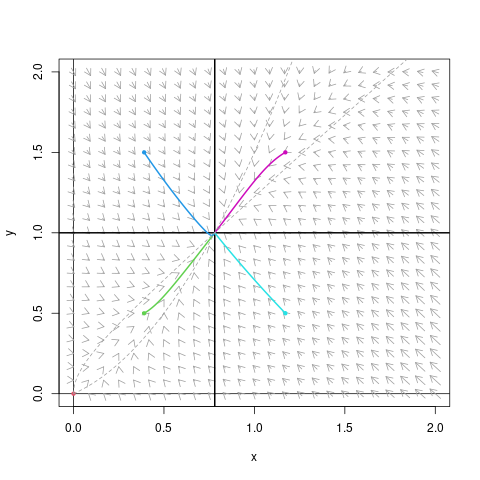
\includegraphics[width=.5\textwidth]{DynPopMaleFemelleCouple.png}
  $$
  }
\end{enumerate}



%-------------------------------------------------------------------------------
\subsubsection{Chemostat}
%-------------------------------------------------------------------------------

Voir \url{https://umr5558-shiny.univ-lyon1.fr/web/}




\newpage \section{Probabilités} %-------------------------------------------------------------------------------
\subsection{Chaînes de Markov}
%-------------------------------------------------------------------------------

%-------------------------------------------------------------------------------
\begin{exercise}[Chaîne de Markov] \label{exo:ChaineMarkov}
  On considère une chaîne de Markov $(X_n)_{n \geq 0}$ prenant ses valeurs dans $\{1, 2, 3, 4\}$, et on note $p(i, j)$ la probabilité de transition de $i$ à $j$. On suppose que $p(1, 1) = p(4, 4) = 1$, que $p(2, 3) = 1 - p(2, 1) =: p$ et que $p(3, 2) = 1 - p(3, 4) =: q$.
  \begin{enumerate}
   \item Donner la matrice de transition de cette chaîne de Markov.
   \item Quelles sont les classes de communication de cette chaîne ? Donner leur nature. Quels sont les comportements asymptotiques possibles de cette chaîne ?
   \item On appelle $x_i$ la probabilité que la chaîne soit absorbée en 1 sachant que $X_0 = i$. Donner $x_1$ et $x_4$, ainsi que deux équations reliant $x_2$ et $x_3$, puis les calculer.
  \end{enumerate}
\end{exercise}

\solution{
  \begin{enumerate}
    \item La matrice de transiiton est
    $$
    P = \left( \begin{array}{cccc}
                1 & 0 & 0 & 0 \\
                1-p & 0 & p & 0 \\
                0 & q & 0 & 1-q \\
                0 & 0 & 0 & 1
              \end{array} \right)
    $$
    \item Les classes de communications sont 
    $$
    C_1 = \{1\}, \qquad C_2 = \{2, 3\}, \qquad C_3 = \{4\}.
    $$
    $C_1$ et $C_3$ sont absorbantes, $C_2$ est transiente. \\
    La chaîne finit nécessairement par être absorbé en 1 ou 4.
    \item D'après la question précédente, on a 
    $$
    x_1 = 1, \qquad x_4 = 0.
    $$
    Pour être absorbé en 1 partant de 3, la chaîne doit d'abord passer de 3 en 2 (avec probabilité $q$), puis être absorbée en 1 partant de 2, donc
    $$
    x_3 = q x_2.
    $$
    Partant de 2 la chaîne peut être immédiatement absorbée en 1 (avec probabilité $1-p$) ou passer en 3 (avec probabilité $p$), puis être absorbée en 1 depuis 3, donc
    $$
    x_2 = (1 - p) + p x_3.
    $$
    $x_2$ vérifie donc
    $$
    x_2 = (1 - p) + p q x_2 
    \qquad \Leftrightarrow \qquad x_2 = \frac{1-p}{1 - pq}
    \qquad \Rightarrow \qquad x_3 = \frac{q(1-p)}{1 - pq}.
    $$
    On peut aussi calculer directement $x_2$ en définissant le temps d'atteinte de l'état $1$ depuis l'état $2$:
    $$
    T_{21} = \inf\{t: X_t = 1 \mid X_0 = 2\}.
    $$
    On remarque alors que, pour $k \geq 0$,  
    $$
    \Pr\{T_{21} = 2k\} = 0, \qquad \Pr\{T_{21} = 2k + 1\} = (1-p) \; (pq)^k
    $$
    et on en déduit
    $$
    x_2 = \sum_{n \geq 0} \Pr\{T_{21} = n\} = \sum_{k \geq 0} \Pr\{T_{21} = 2k+1\} 
    = (1-p) \sum_{k \geq 0} (pq)^k = \frac{1-p}{1 - pq}.
    $$
    De même, on peut déterminer $x_3$ directement à partir de la loi du temps d'atteinte $T_{31}$.
  \end{enumerate}
}

%-------------------------------------------------------------------------------
\begin{exercise}[Processus de branchement] \label{exo:Proba-BGWgeometrique}
  On considère un processus de Bienaymé-Galton-Watson partant d'une population de taille 1 et dans laquelle le nombre de descendants par individu suit une loi géométrique $\Gcal(a)$ (pour mémoire, $X \sim \Gcal(a)$ ssi $\Pr\{X = k\} = (1-a) a^k$).
  \begin{enumerate}
    \item Calculer le nombre moyen $m$ de descendants par individus en fonction de $a$.
    \item Pour quelles valeurs de $a$ le processus est-il critique, sous-critique ou sur-critique ?
    \item Montrer que, pour $m > 1$, la probabilité d'extinction $q$ de cette population vaut $1/m$.
  \end{enumerate}
\end{exercise}

\solution{
  \begin{enumerate}
    \item On a
    $$
    m = \Esp(X) 
    = \sum_{k \geq 0} (1-a) \; a^k \; k 
    = a(1-a) \sum_{k \geq 0} k \; a^{k-1}
    $$
    où on reconnaît la dérivée de la fonction $f(a) = \sum_{k \geq 0} a^{k} = (1-a)^{-1}$, soit $f'(a) = (1-a)^{-2}$. On a donc
    $$
    m
    = a(1-a) (1-a)^{-2}
    = a / (1-a)
    $$
    (qui est une fonction monotone croissante de $a$).
    \item On a $m \leq 1 \; \Leftrightarrow \; a \leq 1-a \; \Leftrightarrow \; a \leq 1/2$.  Le processus est donc critique pour $a = 1/2$, sous critique pour $a < 1/2$ et sur-critique pour $a > 1/2$.
    \item On sait que la probabilité d'extinction $q$ partant d'une population de taille 1 est le plus petit point fixe de l'équation $s = f_X(s)$ où $f_X$ est la fonction génératrice des probabilités de la loi géométrique : 
    $$
    f_X(s) = (1 - a) / (1 - as).
    $$
    On cherche donc à résoudre $1 - a = (1 - as) s \; \Leftrightarrow \; as^2 - s + (1-a) = 0$ dont on sait que $s = 1$ est solution. On peut donc factoriser
    $$
    as^2 - s + (1-a) = a (s-1) \left(s  - \frac{1-a}a\right)
    $$
    où $(1-a)/a < 1$ dès que $a > 1/2$. La probabilité d'extinction vaut donc
    $$
    q = \frac{1-a}a = \frac1m.
    $$
  \end{enumerate}
}
  
%-------------------------------------------------------------------------------
\begin{exercise}[Fonction génératrice] \label{exo:Proba-Generatrice}
  Soit $(X, Y)$ un couple de variables aléatoires entières et $\phi: [0, 1] \times [0, 1] \mapsto [0, 1]$ sa fonction génératrice de $(X, Y)$ définie par 
  $$
  \phi(s, t) = \Esp(s^X t^Y) = \sum_{x \geq 0} \sum_{y geq 0} \Pr\{X=x, Y=y\} \; s^x \; t^y.
  $$
  \begin{enumerate}
   \item Que valent $\phi(1, 1)$, $\phi(1, 0)$, $\phi(0, 1)$ et $\phi(0, 0)$ ?
   \item Exprimer les fonctions génératrices de $X$, de $Y$ et de $X+Y$ en fonction de $\phi$.
   \item Montrer que, si $X$ et $Y$ sont indépendantes, alors $\phi(s, t) = \phi(s, 1) \; \phi(1, t)$.
   \item Montrer que si les couples $(X_1, Y_1)$ et $(X_2, Y_2)$ ont pour fonctions génératrices respectives $\phi_1$ et $\phi_2$, alors le couple $(X_1+X_2, Y_1+Y_2)$ a pour fonction génératrice $\psi = \phi_1 \phi_2$. 
   \item En déduire que si $N$ est une variable aléatoire entière de fonction génératrice $f$ et que $((X_i, Y_i))_{i \geq 1}$ sont des couples i.i.d. de même fonction génératrice $\phi$, alors le couple $(U, V)$ tel que
   $$
   U = \sum_{i=1}^N X_i, \qquad V = \sum_{i=1}^N Y_i
   $$
   a pour fonction génératrice $f \circ \phi$.
  \end{enumerate}
\end{exercise}

\solution{\todo{}}


% %-------------------------------------------------------------------------------
% \bibliography{/home/robin/Biblio/BibGene}
% \bibliographystyle{plainnat}

%-------------------------------------------------------------------------------
%-------------------------------------------------------------------------------
\end{document}
%-------------------------------------------------------------------------------
%-------------------------------------------------------------------------------


